\documentclass[11pt]{article}

    \usepackage[breakable]{tcolorbox}
    \usepackage{parskip} % Stop auto-indenting (to mimic markdown behaviour)
    

    % Basic figure setup, for now with no caption control since it's done
    % automatically by Pandoc (which extracts ![](path) syntax from Markdown).
    \usepackage{graphicx}
    % Maintain compatibility with old templates. Remove in nbconvert 6.0
    \let\Oldincludegraphics\includegraphics
    % Ensure that by default, figures have no caption (until we provide a
    % proper Figure object with a Caption API and a way to capture that
    % in the conversion process - todo).
    \usepackage{caption}
    \DeclareCaptionFormat{nocaption}{}
    \captionsetup{format=nocaption,aboveskip=0pt,belowskip=0pt}

    \usepackage{float}
    \floatplacement{figure}{H} % forces figures to be placed at the correct location
    \usepackage{xcolor} % Allow colors to be defined
    \usepackage{enumerate} % Needed for markdown enumerations to work
    \usepackage{geometry} % Used to adjust the document margins
    \usepackage{amsmath} % Equations
    \usepackage{amssymb} % Equations
    \usepackage{textcomp} % defines textquotesingle
    % Hack from http://tex.stackexchange.com/a/47451/13684:
    \AtBeginDocument{%
        \def\PYZsq{\textquotesingle}% Upright quotes in Pygmentized code
    }
    \usepackage{upquote} % Upright quotes for verbatim code
    \usepackage{eurosym} % defines \euro

    \usepackage{iftex}
    \ifPDFTeX
        \usepackage[T1]{fontenc}
        \IfFileExists{alphabeta.sty}{
              \usepackage{alphabeta}
          }{
              \usepackage[mathletters]{ucs}
              \usepackage[utf8x]{inputenc}
          }
    \else
        \usepackage{fontspec}
        \usepackage{unicode-math}
    \fi

    \usepackage{fancyvrb} % verbatim replacement that allows latex
    \usepackage{grffile} % extends the file name processing of package graphics
                         % to support a larger range
    \makeatletter % fix for old versions of grffile with XeLaTeX
    \@ifpackagelater{grffile}{2019/11/01}
    {
      % Do nothing on new versions
    }
    {
      \def\Gread@@xetex#1{%
        \IfFileExists{"\Gin@base".bb}%
        {\Gread@eps{\Gin@base.bb}}%
        {\Gread@@xetex@aux#1}%
      }
    }
    \makeatother
    \usepackage[Export]{adjustbox} % Used to constrain images to a maximum size
    \adjustboxset{max size={0.9\linewidth}{0.9\paperheight}}

    % The hyperref package gives us a pdf with properly built
    % internal navigation ('pdf bookmarks' for the table of contents,
    % internal cross-reference links, web links for URLs, etc.)
    \usepackage{hyperref}
    % The default LaTeX title has an obnoxious amount of whitespace. By default,
    % titling removes some of it. It also provides customization options.
    \usepackage{titling}
    \usepackage{longtable} % longtable support required by pandoc >1.10
    \usepackage{booktabs}  % table support for pandoc > 1.12.2
    \usepackage{array}     % table support for pandoc >= 2.11.3
    \usepackage{calc}      % table minipage width calculation for pandoc >= 2.11.1
    \usepackage[inline]{enumitem} % IRkernel/repr support (it uses the enumerate* environment)
    \usepackage[normalem]{ulem} % ulem is needed to support strikethroughs (\sout)
                                % normalem makes italics be italics, not underlines
    \usepackage{soul}      % strikethrough (\st) support for pandoc >= 3.0.0
    \usepackage{mathrsfs}
    

    
    % Colors for the hyperref package
    \definecolor{urlcolor}{rgb}{0,.145,.698}
    \definecolor{linkcolor}{rgb}{.71,0.21,0.01}
    \definecolor{citecolor}{rgb}{.12,.54,.11}

    % ANSI colors
    \definecolor{ansi-black}{HTML}{3E424D}
    \definecolor{ansi-black-intense}{HTML}{282C36}
    \definecolor{ansi-red}{HTML}{E75C58}
    \definecolor{ansi-red-intense}{HTML}{B22B31}
    \definecolor{ansi-green}{HTML}{00A250}
    \definecolor{ansi-green-intense}{HTML}{007427}
    \definecolor{ansi-yellow}{HTML}{DDB62B}
    \definecolor{ansi-yellow-intense}{HTML}{B27D12}
    \definecolor{ansi-blue}{HTML}{208FFB}
    \definecolor{ansi-blue-intense}{HTML}{0065CA}
    \definecolor{ansi-magenta}{HTML}{D160C4}
    \definecolor{ansi-magenta-intense}{HTML}{A03196}
    \definecolor{ansi-cyan}{HTML}{60C6C8}
    \definecolor{ansi-cyan-intense}{HTML}{258F8F}
    \definecolor{ansi-white}{HTML}{C5C1B4}
    \definecolor{ansi-white-intense}{HTML}{A1A6B2}
    \definecolor{ansi-default-inverse-fg}{HTML}{FFFFFF}
    \definecolor{ansi-default-inverse-bg}{HTML}{000000}

    % common color for the border for error outputs.
    \definecolor{outerrorbackground}{HTML}{FFDFDF}

    % commands and environments needed by pandoc snippets
    % extracted from the output of `pandoc -s`
    \providecommand{\tightlist}{%
      \setlength{\itemsep}{0pt}\setlength{\parskip}{0pt}}
    \DefineVerbatimEnvironment{Highlighting}{Verbatim}{commandchars=\\\{\}}
    % Add ',fontsize=\small' for more characters per line
    \newenvironment{Shaded}{}{}
    \newcommand{\KeywordTok}[1]{\textcolor[rgb]{0.00,0.44,0.13}{\textbf{{#1}}}}
    \newcommand{\DataTypeTok}[1]{\textcolor[rgb]{0.56,0.13,0.00}{{#1}}}
    \newcommand{\DecValTok}[1]{\textcolor[rgb]{0.25,0.63,0.44}{{#1}}}
    \newcommand{\BaseNTok}[1]{\textcolor[rgb]{0.25,0.63,0.44}{{#1}}}
    \newcommand{\FloatTok}[1]{\textcolor[rgb]{0.25,0.63,0.44}{{#1}}}
    \newcommand{\CharTok}[1]{\textcolor[rgb]{0.25,0.44,0.63}{{#1}}}
    \newcommand{\StringTok}[1]{\textcolor[rgb]{0.25,0.44,0.63}{{#1}}}
    \newcommand{\CommentTok}[1]{\textcolor[rgb]{0.38,0.63,0.69}{\textit{{#1}}}}
    \newcommand{\OtherTok}[1]{\textcolor[rgb]{0.00,0.44,0.13}{{#1}}}
    \newcommand{\AlertTok}[1]{\textcolor[rgb]{1.00,0.00,0.00}{\textbf{{#1}}}}
    \newcommand{\FunctionTok}[1]{\textcolor[rgb]{0.02,0.16,0.49}{{#1}}}
    \newcommand{\RegionMarkerTok}[1]{{#1}}
    \newcommand{\ErrorTok}[1]{\textcolor[rgb]{1.00,0.00,0.00}{\textbf{{#1}}}}
    \newcommand{\NormalTok}[1]{{#1}}

    % Additional commands for more recent versions of Pandoc
    \newcommand{\ConstantTok}[1]{\textcolor[rgb]{0.53,0.00,0.00}{{#1}}}
    \newcommand{\SpecialCharTok}[1]{\textcolor[rgb]{0.25,0.44,0.63}{{#1}}}
    \newcommand{\VerbatimStringTok}[1]{\textcolor[rgb]{0.25,0.44,0.63}{{#1}}}
    \newcommand{\SpecialStringTok}[1]{\textcolor[rgb]{0.73,0.40,0.53}{{#1}}}
    \newcommand{\ImportTok}[1]{{#1}}
    \newcommand{\DocumentationTok}[1]{\textcolor[rgb]{0.73,0.13,0.13}{\textit{{#1}}}}
    \newcommand{\AnnotationTok}[1]{\textcolor[rgb]{0.38,0.63,0.69}{\textbf{\textit{{#1}}}}}
    \newcommand{\CommentVarTok}[1]{\textcolor[rgb]{0.38,0.63,0.69}{\textbf{\textit{{#1}}}}}
    \newcommand{\VariableTok}[1]{\textcolor[rgb]{0.10,0.09,0.49}{{#1}}}
    \newcommand{\ControlFlowTok}[1]{\textcolor[rgb]{0.00,0.44,0.13}{\textbf{{#1}}}}
    \newcommand{\OperatorTok}[1]{\textcolor[rgb]{0.40,0.40,0.40}{{#1}}}
    \newcommand{\BuiltInTok}[1]{{#1}}
    \newcommand{\ExtensionTok}[1]{{#1}}
    \newcommand{\PreprocessorTok}[1]{\textcolor[rgb]{0.74,0.48,0.00}{{#1}}}
    \newcommand{\AttributeTok}[1]{\textcolor[rgb]{0.49,0.56,0.16}{{#1}}}
    \newcommand{\InformationTok}[1]{\textcolor[rgb]{0.38,0.63,0.69}{\textbf{\textit{{#1}}}}}
    \newcommand{\WarningTok}[1]{\textcolor[rgb]{0.38,0.63,0.69}{\textbf{\textit{{#1}}}}}


    % Define a nice break command that doesn't care if a line doesn't already
    % exist.
    \def\br{\hspace*{\fill} \\* }
    % Math Jax compatibility definitions
    \def\gt{>}
    \def\lt{<}
    \let\Oldtex\TeX
    \let\Oldlatex\LaTeX
    \renewcommand{\TeX}{\textrm{\Oldtex}}
    \renewcommand{\LaTeX}{\textrm{\Oldlatex}}
    % Document parameters
    % Document title
    \title{exploring\_word\_vectors\_22\_23}
    
    
    
    
    
    
    
% Pygments definitions
\makeatletter
\def\PY@reset{\let\PY@it=\relax \let\PY@bf=\relax%
    \let\PY@ul=\relax \let\PY@tc=\relax%
    \let\PY@bc=\relax \let\PY@ff=\relax}
\def\PY@tok#1{\csname PY@tok@#1\endcsname}
\def\PY@toks#1+{\ifx\relax#1\empty\else%
    \PY@tok{#1}\expandafter\PY@toks\fi}
\def\PY@do#1{\PY@bc{\PY@tc{\PY@ul{%
    \PY@it{\PY@bf{\PY@ff{#1}}}}}}}
\def\PY#1#2{\PY@reset\PY@toks#1+\relax+\PY@do{#2}}

\@namedef{PY@tok@w}{\def\PY@tc##1{\textcolor[rgb]{0.73,0.73,0.73}{##1}}}
\@namedef{PY@tok@c}{\let\PY@it=\textit\def\PY@tc##1{\textcolor[rgb]{0.24,0.48,0.48}{##1}}}
\@namedef{PY@tok@cp}{\def\PY@tc##1{\textcolor[rgb]{0.61,0.40,0.00}{##1}}}
\@namedef{PY@tok@k}{\let\PY@bf=\textbf\def\PY@tc##1{\textcolor[rgb]{0.00,0.50,0.00}{##1}}}
\@namedef{PY@tok@kp}{\def\PY@tc##1{\textcolor[rgb]{0.00,0.50,0.00}{##1}}}
\@namedef{PY@tok@kt}{\def\PY@tc##1{\textcolor[rgb]{0.69,0.00,0.25}{##1}}}
\@namedef{PY@tok@o}{\def\PY@tc##1{\textcolor[rgb]{0.40,0.40,0.40}{##1}}}
\@namedef{PY@tok@ow}{\let\PY@bf=\textbf\def\PY@tc##1{\textcolor[rgb]{0.67,0.13,1.00}{##1}}}
\@namedef{PY@tok@nb}{\def\PY@tc##1{\textcolor[rgb]{0.00,0.50,0.00}{##1}}}
\@namedef{PY@tok@nf}{\def\PY@tc##1{\textcolor[rgb]{0.00,0.00,1.00}{##1}}}
\@namedef{PY@tok@nc}{\let\PY@bf=\textbf\def\PY@tc##1{\textcolor[rgb]{0.00,0.00,1.00}{##1}}}
\@namedef{PY@tok@nn}{\let\PY@bf=\textbf\def\PY@tc##1{\textcolor[rgb]{0.00,0.00,1.00}{##1}}}
\@namedef{PY@tok@ne}{\let\PY@bf=\textbf\def\PY@tc##1{\textcolor[rgb]{0.80,0.25,0.22}{##1}}}
\@namedef{PY@tok@nv}{\def\PY@tc##1{\textcolor[rgb]{0.10,0.09,0.49}{##1}}}
\@namedef{PY@tok@no}{\def\PY@tc##1{\textcolor[rgb]{0.53,0.00,0.00}{##1}}}
\@namedef{PY@tok@nl}{\def\PY@tc##1{\textcolor[rgb]{0.46,0.46,0.00}{##1}}}
\@namedef{PY@tok@ni}{\let\PY@bf=\textbf\def\PY@tc##1{\textcolor[rgb]{0.44,0.44,0.44}{##1}}}
\@namedef{PY@tok@na}{\def\PY@tc##1{\textcolor[rgb]{0.41,0.47,0.13}{##1}}}
\@namedef{PY@tok@nt}{\let\PY@bf=\textbf\def\PY@tc##1{\textcolor[rgb]{0.00,0.50,0.00}{##1}}}
\@namedef{PY@tok@nd}{\def\PY@tc##1{\textcolor[rgb]{0.67,0.13,1.00}{##1}}}
\@namedef{PY@tok@s}{\def\PY@tc##1{\textcolor[rgb]{0.73,0.13,0.13}{##1}}}
\@namedef{PY@tok@sd}{\let\PY@it=\textit\def\PY@tc##1{\textcolor[rgb]{0.73,0.13,0.13}{##1}}}
\@namedef{PY@tok@si}{\let\PY@bf=\textbf\def\PY@tc##1{\textcolor[rgb]{0.64,0.35,0.47}{##1}}}
\@namedef{PY@tok@se}{\let\PY@bf=\textbf\def\PY@tc##1{\textcolor[rgb]{0.67,0.36,0.12}{##1}}}
\@namedef{PY@tok@sr}{\def\PY@tc##1{\textcolor[rgb]{0.64,0.35,0.47}{##1}}}
\@namedef{PY@tok@ss}{\def\PY@tc##1{\textcolor[rgb]{0.10,0.09,0.49}{##1}}}
\@namedef{PY@tok@sx}{\def\PY@tc##1{\textcolor[rgb]{0.00,0.50,0.00}{##1}}}
\@namedef{PY@tok@m}{\def\PY@tc##1{\textcolor[rgb]{0.40,0.40,0.40}{##1}}}
\@namedef{PY@tok@gh}{\let\PY@bf=\textbf\def\PY@tc##1{\textcolor[rgb]{0.00,0.00,0.50}{##1}}}
\@namedef{PY@tok@gu}{\let\PY@bf=\textbf\def\PY@tc##1{\textcolor[rgb]{0.50,0.00,0.50}{##1}}}
\@namedef{PY@tok@gd}{\def\PY@tc##1{\textcolor[rgb]{0.63,0.00,0.00}{##1}}}
\@namedef{PY@tok@gi}{\def\PY@tc##1{\textcolor[rgb]{0.00,0.52,0.00}{##1}}}
\@namedef{PY@tok@gr}{\def\PY@tc##1{\textcolor[rgb]{0.89,0.00,0.00}{##1}}}
\@namedef{PY@tok@ge}{\let\PY@it=\textit}
\@namedef{PY@tok@gs}{\let\PY@bf=\textbf}
\@namedef{PY@tok@gp}{\let\PY@bf=\textbf\def\PY@tc##1{\textcolor[rgb]{0.00,0.00,0.50}{##1}}}
\@namedef{PY@tok@go}{\def\PY@tc##1{\textcolor[rgb]{0.44,0.44,0.44}{##1}}}
\@namedef{PY@tok@gt}{\def\PY@tc##1{\textcolor[rgb]{0.00,0.27,0.87}{##1}}}
\@namedef{PY@tok@err}{\def\PY@bc##1{{\setlength{\fboxsep}{\string -\fboxrule}\fcolorbox[rgb]{1.00,0.00,0.00}{1,1,1}{\strut ##1}}}}
\@namedef{PY@tok@kc}{\let\PY@bf=\textbf\def\PY@tc##1{\textcolor[rgb]{0.00,0.50,0.00}{##1}}}
\@namedef{PY@tok@kd}{\let\PY@bf=\textbf\def\PY@tc##1{\textcolor[rgb]{0.00,0.50,0.00}{##1}}}
\@namedef{PY@tok@kn}{\let\PY@bf=\textbf\def\PY@tc##1{\textcolor[rgb]{0.00,0.50,0.00}{##1}}}
\@namedef{PY@tok@kr}{\let\PY@bf=\textbf\def\PY@tc##1{\textcolor[rgb]{0.00,0.50,0.00}{##1}}}
\@namedef{PY@tok@bp}{\def\PY@tc##1{\textcolor[rgb]{0.00,0.50,0.00}{##1}}}
\@namedef{PY@tok@fm}{\def\PY@tc##1{\textcolor[rgb]{0.00,0.00,1.00}{##1}}}
\@namedef{PY@tok@vc}{\def\PY@tc##1{\textcolor[rgb]{0.10,0.09,0.49}{##1}}}
\@namedef{PY@tok@vg}{\def\PY@tc##1{\textcolor[rgb]{0.10,0.09,0.49}{##1}}}
\@namedef{PY@tok@vi}{\def\PY@tc##1{\textcolor[rgb]{0.10,0.09,0.49}{##1}}}
\@namedef{PY@tok@vm}{\def\PY@tc##1{\textcolor[rgb]{0.10,0.09,0.49}{##1}}}
\@namedef{PY@tok@sa}{\def\PY@tc##1{\textcolor[rgb]{0.73,0.13,0.13}{##1}}}
\@namedef{PY@tok@sb}{\def\PY@tc##1{\textcolor[rgb]{0.73,0.13,0.13}{##1}}}
\@namedef{PY@tok@sc}{\def\PY@tc##1{\textcolor[rgb]{0.73,0.13,0.13}{##1}}}
\@namedef{PY@tok@dl}{\def\PY@tc##1{\textcolor[rgb]{0.73,0.13,0.13}{##1}}}
\@namedef{PY@tok@s2}{\def\PY@tc##1{\textcolor[rgb]{0.73,0.13,0.13}{##1}}}
\@namedef{PY@tok@sh}{\def\PY@tc##1{\textcolor[rgb]{0.73,0.13,0.13}{##1}}}
\@namedef{PY@tok@s1}{\def\PY@tc##1{\textcolor[rgb]{0.73,0.13,0.13}{##1}}}
\@namedef{PY@tok@mb}{\def\PY@tc##1{\textcolor[rgb]{0.40,0.40,0.40}{##1}}}
\@namedef{PY@tok@mf}{\def\PY@tc##1{\textcolor[rgb]{0.40,0.40,0.40}{##1}}}
\@namedef{PY@tok@mh}{\def\PY@tc##1{\textcolor[rgb]{0.40,0.40,0.40}{##1}}}
\@namedef{PY@tok@mi}{\def\PY@tc##1{\textcolor[rgb]{0.40,0.40,0.40}{##1}}}
\@namedef{PY@tok@il}{\def\PY@tc##1{\textcolor[rgb]{0.40,0.40,0.40}{##1}}}
\@namedef{PY@tok@mo}{\def\PY@tc##1{\textcolor[rgb]{0.40,0.40,0.40}{##1}}}
\@namedef{PY@tok@ch}{\let\PY@it=\textit\def\PY@tc##1{\textcolor[rgb]{0.24,0.48,0.48}{##1}}}
\@namedef{PY@tok@cm}{\let\PY@it=\textit\def\PY@tc##1{\textcolor[rgb]{0.24,0.48,0.48}{##1}}}
\@namedef{PY@tok@cpf}{\let\PY@it=\textit\def\PY@tc##1{\textcolor[rgb]{0.24,0.48,0.48}{##1}}}
\@namedef{PY@tok@c1}{\let\PY@it=\textit\def\PY@tc##1{\textcolor[rgb]{0.24,0.48,0.48}{##1}}}
\@namedef{PY@tok@cs}{\let\PY@it=\textit\def\PY@tc##1{\textcolor[rgb]{0.24,0.48,0.48}{##1}}}

\def\PYZbs{\char`\\}
\def\PYZus{\char`\_}
\def\PYZob{\char`\{}
\def\PYZcb{\char`\}}
\def\PYZca{\char`\^}
\def\PYZam{\char`\&}
\def\PYZlt{\char`\<}
\def\PYZgt{\char`\>}
\def\PYZsh{\char`\#}
\def\PYZpc{\char`\%}
\def\PYZdl{\char`\$}
\def\PYZhy{\char`\-}
\def\PYZsq{\char`\'}
\def\PYZdq{\char`\"}
\def\PYZti{\char`\~}
% for compatibility with earlier versions
\def\PYZat{@}
\def\PYZlb{[}
\def\PYZrb{]}
\makeatother


    % For linebreaks inside Verbatim environment from package fancyvrb.
    \makeatletter
        \newbox\Wrappedcontinuationbox
        \newbox\Wrappedvisiblespacebox
        \newcommand*\Wrappedvisiblespace {\textcolor{red}{\textvisiblespace}}
        \newcommand*\Wrappedcontinuationsymbol {\textcolor{red}{\llap{\tiny$\m@th\hookrightarrow$}}}
        \newcommand*\Wrappedcontinuationindent {3ex }
        \newcommand*\Wrappedafterbreak {\kern\Wrappedcontinuationindent\copy\Wrappedcontinuationbox}
        % Take advantage of the already applied Pygments mark-up to insert
        % potential linebreaks for TeX processing.
        %        {, <, #, %, $, ' and ": go to next line.
        %        _, }, ^, &, >, - and ~: stay at end of broken line.
        % Use of \textquotesingle for straight quote.
        \newcommand*\Wrappedbreaksatspecials {%
            \def\PYGZus{\discretionary{\char`\_}{\Wrappedafterbreak}{\char`\_}}%
            \def\PYGZob{\discretionary{}{\Wrappedafterbreak\char`\{}{\char`\{}}%
            \def\PYGZcb{\discretionary{\char`\}}{\Wrappedafterbreak}{\char`\}}}%
            \def\PYGZca{\discretionary{\char`\^}{\Wrappedafterbreak}{\char`\^}}%
            \def\PYGZam{\discretionary{\char`\&}{\Wrappedafterbreak}{\char`\&}}%
            \def\PYGZlt{\discretionary{}{\Wrappedafterbreak\char`\<}{\char`\<}}%
            \def\PYGZgt{\discretionary{\char`\>}{\Wrappedafterbreak}{\char`\>}}%
            \def\PYGZsh{\discretionary{}{\Wrappedafterbreak\char`\#}{\char`\#}}%
            \def\PYGZpc{\discretionary{}{\Wrappedafterbreak\char`\%}{\char`\%}}%
            \def\PYGZdl{\discretionary{}{\Wrappedafterbreak\char`\$}{\char`\$}}%
            \def\PYGZhy{\discretionary{\char`\-}{\Wrappedafterbreak}{\char`\-}}%
            \def\PYGZsq{\discretionary{}{\Wrappedafterbreak\textquotesingle}{\textquotesingle}}%
            \def\PYGZdq{\discretionary{}{\Wrappedafterbreak\char`\"}{\char`\"}}%
            \def\PYGZti{\discretionary{\char`\~}{\Wrappedafterbreak}{\char`\~}}%
        }
        % Some characters . , ; ? ! / are not pygmentized.
        % This macro makes them "active" and they will insert potential linebreaks
        \newcommand*\Wrappedbreaksatpunct {%
            \lccode`\~`\.\lowercase{\def~}{\discretionary{\hbox{\char`\.}}{\Wrappedafterbreak}{\hbox{\char`\.}}}%
            \lccode`\~`\,\lowercase{\def~}{\discretionary{\hbox{\char`\,}}{\Wrappedafterbreak}{\hbox{\char`\,}}}%
            \lccode`\~`\;\lowercase{\def~}{\discretionary{\hbox{\char`\;}}{\Wrappedafterbreak}{\hbox{\char`\;}}}%
            \lccode`\~`\:\lowercase{\def~}{\discretionary{\hbox{\char`\:}}{\Wrappedafterbreak}{\hbox{\char`\:}}}%
            \lccode`\~`\?\lowercase{\def~}{\discretionary{\hbox{\char`\?}}{\Wrappedafterbreak}{\hbox{\char`\?}}}%
            \lccode`\~`\!\lowercase{\def~}{\discretionary{\hbox{\char`\!}}{\Wrappedafterbreak}{\hbox{\char`\!}}}%
            \lccode`\~`\/\lowercase{\def~}{\discretionary{\hbox{\char`\/}}{\Wrappedafterbreak}{\hbox{\char`\/}}}%
            \catcode`\.\active
            \catcode`\,\active
            \catcode`\;\active
            \catcode`\:\active
            \catcode`\?\active
            \catcode`\!\active
            \catcode`\/\active
            \lccode`\~`\~
        }
    \makeatother

    \let\OriginalVerbatim=\Verbatim
    \makeatletter
    \renewcommand{\Verbatim}[1][1]{%
        %\parskip\z@skip
        \sbox\Wrappedcontinuationbox {\Wrappedcontinuationsymbol}%
        \sbox\Wrappedvisiblespacebox {\FV@SetupFont\Wrappedvisiblespace}%
        \def\FancyVerbFormatLine ##1{\hsize\linewidth
            \vtop{\raggedright\hyphenpenalty\z@\exhyphenpenalty\z@
                \doublehyphendemerits\z@\finalhyphendemerits\z@
                \strut ##1\strut}%
        }%
        % If the linebreak is at a space, the latter will be displayed as visible
        % space at end of first line, and a continuation symbol starts next line.
        % Stretch/shrink are however usually zero for typewriter font.
        \def\FV@Space {%
            \nobreak\hskip\z@ plus\fontdimen3\font minus\fontdimen4\font
            \discretionary{\copy\Wrappedvisiblespacebox}{\Wrappedafterbreak}
            {\kern\fontdimen2\font}%
        }%

        % Allow breaks at special characters using \PYG... macros.
        \Wrappedbreaksatspecials
        % Breaks at punctuation characters . , ; ? ! and / need catcode=\active
        \OriginalVerbatim[#1,codes*=\Wrappedbreaksatpunct]%
    }
    \makeatother

    % Exact colors from NB
    \definecolor{incolor}{HTML}{303F9F}
    \definecolor{outcolor}{HTML}{D84315}
    \definecolor{cellborder}{HTML}{CFCFCF}
    \definecolor{cellbackground}{HTML}{F7F7F7}

    % prompt
    \makeatletter
    \newcommand{\boxspacing}{\kern\kvtcb@left@rule\kern\kvtcb@boxsep}
    \makeatother
    \newcommand{\prompt}[4]{
        {\ttfamily\llap{{\color{#2}[#3]:\hspace{3pt}#4}}\vspace{-\baselineskip}}
    }
    

    
    % Prevent overflowing lines due to hard-to-break entities
    \sloppy
    % Setup hyperref package
    \hypersetup{
      breaklinks=true,  % so long urls are correctly broken across lines
      colorlinks=true,
      urlcolor=urlcolor,
      linkcolor=linkcolor,
      citecolor=citecolor,
      }
    % Slightly bigger margins than the latex defaults
    
    \geometry{verbose,tmargin=1in,bmargin=1in,lmargin=1in,rmargin=1in}
    
    

\begin{document}

\maketitle




\section{CS224N Assignment 1: Exploring Word Vectors (25
  Points)}\label{cs224n-assignment-1-exploring-word-vectors-25-points}

\subsubsection{\texorpdfstring{ Due 4:30pm, Tue Jan 17
    }{ Due 4:30pm, Tue Jan 17 }}\label{due-430pm-tue-jan-17}

Welcome to CS224N!

Before you start, make sure you read the README.txt in the same
directory as this notebook for important setup information. A lot of
code is provided in this notebook, and we highly encourage you to read
and understand it as part of the learning :)

If you aren't super familiar with Python, Numpy, or Matplotlib, we
recommend you check out the review session on Friday. The session will
be recorded and the material will be made available on our
\href{http://web.stanford.edu/class/cs224n/index.html\#schedule}{website}.
The CS231N Python/Numpy
\href{https://cs231n.github.io/python-numpy-tutorial/}{tutorial} is also
a great resource.

\textbf{Assignment Notes:} Please make sure to save the notebook as you
go along. Submission Instructions are located at the bottom of the
notebook.

\begin{tcolorbox}[breakable, size=fbox, boxrule=1pt, pad at break*=1mm,colback=cellbackground, colframe=cellborder]
    \prompt{In}{incolor}{70}{\boxspacing}
    \begin{Verbatim}[commandchars=\\\{\}]
        \PY{c+c1}{\PYZsh{} All Import Statements Defined Here}
        \PY{c+c1}{\PYZsh{} Note: Do not add to this list.}
        \PY{c+c1}{\PYZsh{} \PYZhy{}\PYZhy{}\PYZhy{}\PYZhy{}\PYZhy{}\PYZhy{}\PYZhy{}\PYZhy{}\PYZhy{}\PYZhy{}\PYZhy{}\PYZhy{}\PYZhy{}\PYZhy{}\PYZhy{}\PYZhy{}}

        \PY{k+kn}{import} \PY{n+nn}{sys}
        \PY{k}{assert} \PY{n}{sys}\PY{o}{.}\PY{n}{version\PYZus{}info}\PY{p}{[}\PY{l+m+mi}{0}\PY{p}{]}\PY{o}{==}\PY{l+m+mi}{3}
        \PY{k}{assert} \PY{n}{sys}\PY{o}{.}\PY{n}{version\PYZus{}info}\PY{p}{[}\PY{l+m+mi}{1}\PY{p}{]} \PY{o}{\PYZgt{}}\PY{o}{=} \PY{l+m+mi}{5}

        \PY{k+kn}{from} \PY{n+nn}{platform} \PY{k+kn}{import} \PY{n}{python\PYZus{}version}
        \PY{k}{assert} \PY{n+nb}{int}\PY{p}{(}\PY{n}{python\PYZus{}version}\PY{p}{(}\PY{p}{)}\PY{o}{.}\PY{n}{split}\PY{p}{(}\PY{l+s+s2}{\PYZdq{}}\PY{l+s+s2}{.}\PY{l+s+s2}{\PYZdq{}}\PY{p}{)}\PY{p}{[}\PY{l+m+mi}{1}\PY{p}{]}\PY{p}{)} \PY{o}{\PYZgt{}}\PY{o}{=} \PY{l+m+mi}{5}\PY{p}{,} \PY{l+s+s2}{\PYZdq{}}\PY{l+s+s2}{Please upgrade your Python version following the instructions in }\PY{l+s+se}{\PYZbs{}}
        \PY{l+s+s2}{    the README.txt file found in the same directory as this notebook. Your Python version is }\PY{l+s+s2}{\PYZdq{}} \PY{o}{+} \PY{n}{python\PYZus{}version}\PY{p}{(}\PY{p}{)}

        \PY{k+kn}{from} \PY{n+nn}{gensim}\PY{n+nn}{.}\PY{n+nn}{models} \PY{k+kn}{import} \PY{n}{KeyedVectors}
        \PY{k+kn}{from} \PY{n+nn}{gensim}\PY{n+nn}{.}\PY{n+nn}{test}\PY{n+nn}{.}\PY{n+nn}{utils} \PY{k+kn}{import} \PY{n}{datapath}
        \PY{k+kn}{import} \PY{n+nn}{pprint}
        \PY{k+kn}{import} \PY{n+nn}{matplotlib}\PY{n+nn}{.}\PY{n+nn}{pyplot} \PY{k}{as} \PY{n+nn}{plt}
        \PY{n}{plt}\PY{o}{.}\PY{n}{rcParams}\PY{p}{[}\PY{l+s+s1}{\PYZsq{}}\PY{l+s+s1}{figure.figsize}\PY{l+s+s1}{\PYZsq{}}\PY{p}{]} \PY{o}{=} \PY{p}{[}\PY{l+m+mi}{10}\PY{p}{,} \PY{l+m+mi}{5}\PY{p}{]}

        \PY{k+kn}{import} \PY{n+nn}{nltk}
        \PY{n}{nltk}\PY{o}{.}\PY{n}{download}\PY{p}{(}\PY{l+s+s1}{\PYZsq{}}\PY{l+s+s1}{reuters}\PY{l+s+s1}{\PYZsq{}}\PY{p}{,} \PY{n}{download\PYZus{}dir}\PY{o}{=}\PY{l+s+s1}{\PYZsq{}}\PY{l+s+s1}{./data}\PY{l+s+s1}{\PYZsq{}}\PY{p}{)} \PY{c+c1}{\PYZsh{}to specify download location, optionally add the argument: download\PYZus{}dir=\PYZsq{}/specify/desired/path/\PYZsq{}}
        \PY{k+kn}{from} \PY{n+nn}{nltk}\PY{n+nn}{.}\PY{n+nn}{corpus} \PY{k+kn}{import} \PY{n}{reuters}

        \PY{k+kn}{import} \PY{n+nn}{numpy} \PY{k}{as} \PY{n+nn}{np}
        \PY{k+kn}{import} \PY{n+nn}{random}
        \PY{k+kn}{import} \PY{n+nn}{scipy} \PY{k}{as} \PY{n+nn}{sp}
        \PY{k+kn}{from} \PY{n+nn}{sklearn}\PY{n+nn}{.}\PY{n+nn}{decomposition} \PY{k+kn}{import} \PY{n}{TruncatedSVD}
        \PY{k+kn}{from} \PY{n+nn}{sklearn}\PY{n+nn}{.}\PY{n+nn}{decomposition} \PY{k+kn}{import} \PY{n}{PCA}

        \PY{n}{START\PYZus{}TOKEN} \PY{o}{=} \PY{l+s+s1}{\PYZsq{}}\PY{l+s+s1}{\PYZlt{}START\PYZgt{}}\PY{l+s+s1}{\PYZsq{}}
        \PY{n}{END\PYZus{}TOKEN} \PY{o}{=} \PY{l+s+s1}{\PYZsq{}}\PY{l+s+s1}{\PYZlt{}END\PYZgt{}}\PY{l+s+s1}{\PYZsq{}}

        \PY{n}{np}\PY{o}{.}\PY{n}{random}\PY{o}{.}\PY{n}{seed}\PY{p}{(}\PY{l+m+mi}{0}\PY{p}{)}
        \PY{n}{random}\PY{o}{.}\PY{n}{seed}\PY{p}{(}\PY{l+m+mi}{0}\PY{p}{)}
        \PY{c+c1}{\PYZsh{} \PYZhy{}\PYZhy{}\PYZhy{}\PYZhy{}\PYZhy{}\PYZhy{}\PYZhy{}\PYZhy{}\PYZhy{}\PYZhy{}\PYZhy{}\PYZhy{}\PYZhy{}\PYZhy{}\PYZhy{}\PYZhy{}}
    \end{Verbatim}
\end{tcolorbox}

\begin{Verbatim}[commandchars=\\\{\}]
    [nltk\_data] Downloading package reuters to ./data{\ldots}
    [nltk\_data]   Package reuters is already up-to-date!
\end{Verbatim}

\subsection{Word Vectors}\label{word-vectors}

Word Vectors are often used as a fundamental component for downstream
NLP tasks, e.g.~question answering, text generation, translation, etc.,
so it is important to build some intuitions as to their strengths and
weaknesses. Here, you will explore two types of word vectors: those
derived from \emph{co-occurrence matrices}, and those derived via
\emph{GloVe}.

\textbf{Note on Terminology:} The terms ``word vectors'' and ``word
embeddings'' are often used interchangeably. The term ``embedding''
refers to the fact that we are encoding aspects of a word's meaning in a
lower dimensional space. As
\href{https://en.wikipedia.org/wiki/Word_embedding}{Wikipedia} states,
``\emph{conceptually it involves a mathematical embedding from a space
    with one dimension per word to a continuous vector space with a much
    lower dimension}''.

\subsection{Part 1: Count-Based Word Vectors (10
    points)}\label{part-1-count-based-word-vectors-10-points}

Most word vector models start from the following idea:

\emph{You shall know a word by the company it keeps
    (\href{https://en.wikipedia.org/wiki/John_Rupert_Firth}{Firth, J. R.
        1957:11})}

Many word vector implementations are driven by the idea that similar
words, i.e., (near) synonyms, will be used in similar contexts. As a
result, similar words will often be spoken or written along with a
shared subset of words, i.e., contexts. By examining these contexts, we
can try to develop embeddings for our words. With this intuition in
mind, many ``old school'' approaches to constructing word vectors relied
on word counts. Here we elaborate upon one of those strategies,
\emph{co-occurrence matrices} (for more information, see
\href{https://web.stanford.edu/~jurafsky/slp3/6.pdf}{here} or
\href{https://medium.com/data-science-group-iitr/word-embedding-2d05d270b285}{here}).

\subsubsection{Co-Occurrence}\label{co-occurrence}

A co-occurrence matrix counts how often things co-occur in some
environment. Given some word \(w_i\) occurring in the document, we
consider the \emph{context window} surrounding \(w_i\). Supposing our
fixed window size is \(n\), then this is the \(n\) preceding and \(n\)
subsequent words in that document, i.e.~words \(w_{i-n} \dots w_{i-1}\)
and \(w_{i+1} \dots w_{i+n}\). We build a \emph{co-occurrence matrix}
\(M\), which is a symmetric word-by-word matrix in which \(M_{ij}\) is
the number of times \(w_j\) appears inside \(w_i\)'s window among all
documents.

\textbf{Example: Co-Occurrence with Fixed Window of n=1}:

Document 1: ``all that glitters is not gold''

Document 2: ``all is well that ends well''

\begin{longtable}[]{@{}
    >{\raggedright\arraybackslash}p{(\linewidth - 20\tabcolsep) * \real{0.1351}}
    >{\raggedright\arraybackslash}p{(\linewidth - 20\tabcolsep) * \real{0.0946}}
    >{\raggedright\arraybackslash}p{(\linewidth - 20\tabcolsep) * \real{0.0676}}
    >{\raggedright\arraybackslash}p{(\linewidth - 20\tabcolsep) * \real{0.0811}}
    >{\raggedright\arraybackslash}p{(\linewidth - 20\tabcolsep) * \real{0.1351}}
    >{\raggedright\arraybackslash}p{(\linewidth - 20\tabcolsep) * \real{0.0811}}
    >{\raggedright\arraybackslash}p{(\linewidth - 20\tabcolsep) * \real{0.0811}}
    >{\raggedright\arraybackslash}p{(\linewidth - 20\tabcolsep) * \real{0.0946}}
    >{\raggedright\arraybackslash}p{(\linewidth - 20\tabcolsep) * \real{0.0811}}
    >{\raggedright\arraybackslash}p{(\linewidth - 20\tabcolsep) * \real{0.0811}}
    >{\raggedright\arraybackslash}p{(\linewidth - 20\tabcolsep) * \real{0.0676}}@{}}
    \toprule\noalign{}
    \begin{minipage}[b]{\linewidth}\raggedright
        *
    \end{minipage} & \begin{minipage}[b]{\linewidth}\raggedright
                         \texttt{\textless{}START\textgreater{}}
                     \end{minipage} & \begin{minipage}[b]{\linewidth}\raggedright
                                          all
                                      \end{minipage} & \begin{minipage}[b]{\linewidth}\raggedright
                                                           that
                                                       \end{minipage} & \begin{minipage}[b]{\linewidth}\raggedright
                                                                            glitters
                                                                        \end{minipage} & \begin{minipage}[b]{\linewidth}\raggedright
                                                                                             is
                                                                                         \end{minipage} & \begin{minipage}[b]{\linewidth}\raggedright
                                                                                                              not
                                                                                                          \end{minipage} & \begin{minipage}[b]{\linewidth}\raggedright
                                                                                                                               gold
                                                                                                                           \end{minipage} & \begin{minipage}[b]{\linewidth}\raggedright
                                                                                                                                                well
                                                                                                                                            \end{minipage} & \begin{minipage}[b]{\linewidth}\raggedright
                                                                                                                                                                 ends
                                                                                                                                                             \end{minipage} & \begin{minipage}[b]{\linewidth}\raggedright
                                                                                                                                                                                  \texttt{\textless{}END\textgreater{}}
                                                                                                                                                                              \end{minipage}                                                                                                                                                                                                                                                            \\
    \midrule\noalign{}
    \endhead
    \bottomrule\noalign{}
    \endlastfoot
    \texttt{\textless{}START\textgreater{}}     & 0                                                                    & 2                                           & 0                                           & 0                                           & 0                                           & 0                                           & 0                                           & 0
                                                & 0                                                                    & 0                                                                                                                                                                                                                                                                                                                                                                                 \\
    all                                         & 2                                                                    & 0                                           & 1                                           & 0                                           & 1                                           & 0                                           & 0                                           & 0                                           & 0                                           & 0 \\
    that                                        & 0                                                                    & 1                                           & 0                                           & 1                                           & 0                                           & 0                                           & 0                                           & 1                                           & 1                                           & 0 \\
    glitters                                    & 0                                                                    & 0                                           & 1                                           & 0                                           & 1                                           & 0                                           & 0                                           & 0                                           & 0                                           & 0 \\
    is                                          & 0                                                                    & 1                                           & 0                                           & 1                                           & 0                                           & 1                                           & 0                                           & 1                                           & 0                                           & 0 \\
    not                                         & 0                                                                    & 0                                           & 0                                           & 0                                           & 1                                           & 0                                           & 1                                           & 0                                           & 0                                           & 0 \\
    gold                                        & 0                                                                    & 0                                           & 0                                           & 0                                           & 0                                           & 1                                           & 0                                           & 0                                           & 0                                           & 1 \\
    well                                        & 0                                                                    & 0                                           & 1                                           & 0                                           & 1                                           & 0                                           & 0                                           & 0                                           & 1                                           & 1 \\
    ends                                        & 0                                                                    & 0                                           & 1                                           & 0                                           & 0                                           & 0                                           & 0                                           & 1                                           & 0                                           & 0 \\
    \texttt{\textless{}END\textgreater{}}       & 0                                                                    & 0                                           & 0                                           & 0                                           & 0                                           & 0                                           & 1                                           & 1                                           &
    0                                           & 0                                                                                                                                                                                                                                                                                                                                                                                                                                                        \\
\end{longtable}

\textbf{Note:} In NLP, we often add
\texttt{\textless{}START\textgreater{}} and
\texttt{\textless{}END\textgreater{}} tokens to represent the beginning
and end of sentences, paragraphs or documents. In this case we imagine
\texttt{\textless{}START\textgreater{}} and
\texttt{\textless{}END\textgreater{}} tokens encapsulating each
document, e.g., ``\texttt{\textless{}START\textgreater{}} All that
glitters is not gold \texttt{\textless{}END\textgreater{}}'', and
include these tokens in our co-occurrence counts.

The rows (or columns) of this matrix provide one type of word vectors
(those based on word-word co-occurrence), but the vectors will be large
in general (linear in the number of distinct words in a corpus). Thus,
our next step is to run \emph{dimensionality reduction}. In particular,
we will run \emph{SVD (Singular Value Decomposition)}, which is a kind
of generalized \emph{PCA (Principal Components Analysis)} to select the
top \(k\) principal components. Here's a visualization of dimensionality
reduction with SVD. In this picture our co-occurrence matrix is \(A\)
with \(n\) rows corresponding to \(n\) words. We obtain a full matrix
decomposition, with the singular values ordered in the diagonal \(S\)
matrix, and our new, shorter length-\(k\) word vectors in \(U_k\).

\begin{figure}
    \centering
    \pandocbounded{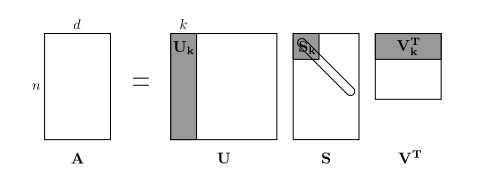
\includegraphics[keepaspectratio]{imgs/svd.png}}
    \caption{Picture of an SVD}
\end{figure}

This reduced-dimensionality co-occurrence representation preserves
semantic relationships between words, e.g.~\emph{doctor} and
\emph{hospital} will be closer than \emph{doctor} and \emph{dog}.

\textbf{Notes:} If you can barely remember what an eigenvalue is, here's
\href{https://davetang.org/file/Singular_Value_Decomposition_Tutorial.pdf}{a
    slow, friendly introduction to SVD}. If you want to learn more
thoroughly about PCA or SVD, feel free to check out lectures
\href{https://web.stanford.edu/class/cs168/l/l7.pdf}{7},
\href{http://theory.stanford.edu/~tim/s15/l/l8.pdf}{8}, and
\href{https://web.stanford.edu/class/cs168/l/l9.pdf}{9} of CS168. These
course notes provide a great high-level treatment of these general
purpose algorithms. Though, for the purpose of this class, you only need
to know how to extract the k-dimensional embeddings by utilizing
pre-programmed implementations of these algorithms from the numpy,
scipy, or sklearn python packages. In practice, it is challenging to
apply full SVD to large corpora because of the memory needed to perform
PCA or SVD. However, if you only want the top \(k\) vector components
for relatively small \(k\) --- known as
\href{https://en.wikipedia.org/wiki/Singular_value_decomposition\#Truncated_SVD}{Truncated
    SVD} --- then there are reasonably scalable techniques to compute those
iteratively.

\subsubsection{Plotting Co-Occurrence Word
    Embeddings}\label{plotting-co-occurrence-word-embeddings}

Here, we will be using the Reuters (business and financial news) corpus.
If you haven't run the import cell at the top of this page, please run
it now (click it and press SHIFT-RETURN). The corpus consists of 10,788
news documents totaling 1.3 million words. These documents span 90
categories and are split into train and test. For more details, please
see https://www.nltk.org/book/ch02.html. We provide a
\texttt{read\_corpus} function below that pulls out only articles from
the ``gold'' (i.e.~news articles about gold, mining, etc.) category. The
function also adds \texttt{\textless{}START\textgreater{}} and
\texttt{\textless{}END\textgreater{}} tokens to each of the documents,
and lowercases words. You do \textbf{not} have to perform any other kind
of pre-processing.

\begin{tcolorbox}[breakable, size=fbox, boxrule=1pt, pad at break*=1mm,colback=cellbackground, colframe=cellborder]
    \prompt{In}{incolor}{71}{\boxspacing}
    \begin{Verbatim}[commandchars=\\\{\}]
        \PY{k}{def} \PY{n+nf}{read\PYZus{}corpus}\PY{p}{(}\PY{n}{category}\PY{o}{=}\PY{l+s+s2}{\PYZdq{}}\PY{l+s+s2}{gold}\PY{l+s+s2}{\PYZdq{}}\PY{p}{)}\PY{p}{:}
        \PY{+w}{    }\PY{l+s+sd}{\PYZdq{}\PYZdq{}\PYZdq{} Read files from the specified Reuter\PYZsq{}s category.}
        \PY{l+s+sd}{        Params:}
        \PY{l+s+sd}{            category (string): category name}
        \PY{l+s+sd}{        Return:}
        \PY{l+s+sd}{            list of lists, with words from each of the processed files}
        \PY{l+s+sd}{    \PYZdq{}\PYZdq{}\PYZdq{}}
        \PY{n}{files} \PY{o}{=} \PY{n}{reuters}\PY{o}{.}\PY{n}{fileids}\PY{p}{(}\PY{n}{category}\PY{p}{)}
        \PY{k}{return} \PY{p}{[}\PY{p}{[}\PY{n}{START\PYZus{}TOKEN}\PY{p}{]} \PY{o}{+} \PY{p}{[}\PY{n}{w}\PY{o}{.}\PY{n}{lower}\PY{p}{(}\PY{p}{)} \PY{k}{for} \PY{n}{w} \PY{o+ow}{in} \PY{n+nb}{list}\PY{p}{(}\PY{n}{reuters}\PY{o}{.}\PY{n}{words}\PY{p}{(}\PY{n}{f}\PY{p}{)}\PY{p}{)}\PY{p}{]} \PY{o}{+} \PY{p}{[}\PY{n}{END\PYZus{}TOKEN}\PY{p}{]} \PY{k}{for} \PY{n}{f} \PY{o+ow}{in} \PY{n}{files}\PY{p}{]}
    \end{Verbatim}
\end{tcolorbox}

Let's have a look what these documents are like\ldots.

\begin{tcolorbox}[breakable, size=fbox, boxrule=1pt, pad at break*=1mm,colback=cellbackground, colframe=cellborder]
    \prompt{In}{incolor}{72}{\boxspacing}
    \begin{Verbatim}[commandchars=\\\{\}]
        \PY{n}{reuters\PYZus{}corpus} \PY{o}{=} \PY{n}{read\PYZus{}corpus}\PY{p}{(}\PY{p}{)}
        \PY{n}{pprint}\PY{o}{.}\PY{n}{pprint}\PY{p}{(}\PY{n}{reuters\PYZus{}corpus}\PY{p}{[}\PY{p}{:}\PY{l+m+mi}{3}\PY{p}{]}\PY{p}{,} \PY{n}{compact}\PY{o}{=}\PY{k+kc}{True}\PY{p}{,} \PY{n}{width}\PY{o}{=}\PY{l+m+mi}{100}\PY{p}{)}
    \end{Verbatim}
\end{tcolorbox}

\begin{Verbatim}[commandchars=\\\{\}]
    [['<START>', 'western', 'mining', 'to', 'open', 'new', 'gold', 'mine', 'in',
            'australia', 'western',
            'mining', 'corp', 'holdings', 'ltd', '\&', 'lt', ';', 'wmng', '.', 's', '>',
            '(', 'wmc', ')',
            'said', 'it', 'will', 'establish', 'a', 'new', 'joint', 'venture', 'gold',
            'mine', 'in', 'the',
            'northern', 'territory', 'at', 'a', 'cost', 'of', 'about', '21', 'mln',
            'dlrs', '.', 'the',
            'mine', ',', 'to', 'be', 'known', 'as', 'the', 'goodall', 'project', ',',
            'will', 'be', 'owned',
            '60', 'pct', 'by', 'wmc', 'and', '40', 'pct', 'by', 'a', 'local', 'w', '.',
            'r', '.', 'grace',
            'and', 'co', '\&', 'lt', ';', 'gra', '>', 'unit', '.', 'it', 'is', 'located',
            '30', 'kms', 'east',
            'of', 'the', 'adelaide', 'river', 'at', 'mt', '.', 'bundey', ',', 'wmc',
            'said', 'in', 'a',
            'statement', 'it', 'said', 'the', 'open', '-', 'pit', 'mine', ',', 'with',
            'a', 'conventional',
            'leach', 'treatment', 'plant', ',', 'is', 'expected', 'to', 'produce',
            'about', '50', ',', '000',
            'ounces', 'of', 'gold', 'in', 'its', 'first', 'year', 'of', 'production',
            'from', 'mid', '-',
            '1988', '.', 'annual', 'ore', 'capacity', 'will', 'be', 'about', '750', ',',
            '000', 'tonnes', '.',
            '<END>'],
    ['<START>', 'belgium', 'to', 'issue', 'gold', 'warrants', ',', 'sources',
            'say', 'belgium',
            'plans', 'to', 'issue', 'swiss', 'franc', 'warrants', 'to', 'buy', 'gold',
            ',', 'with', 'credit',
            'suisse', 'as', 'lead', 'manager', ',', 'market', 'sources', 'said', '.',
            'no', 'confirmation',
            'or', 'further', 'details', 'were', 'immediately', 'available', '.', '<END>'],
    ['<START>', 'belgium', 'launches', 'bonds', 'with', 'gold', 'warrants', 'the',
            'kingdom', 'of',
            'belgium', 'is', 'launching', '100', 'mln', 'swiss', 'francs', 'of', 'seven',
            'year', 'notes',
            'with', 'warrants', 'attached', 'to', 'buy', 'gold', ',', 'lead', 'mananger',
            'credit', 'suisse',
            'said', '.', 'the', 'notes', 'themselves', 'have', 'a', '3', '-', '3', '/',
            '8', 'pct', 'coupon',
            'and', 'are', 'priced', 'at', 'par', '.', 'payment', 'is', 'due', 'april',
            '30', ',', '1987',
            'and', 'final', 'maturity', 'april', '30', ',', '1994', '.', 'each', '50',
            ',', '000', 'franc',
            'note', 'carries', '15', 'warrants', '.', 'two', 'warrants', 'are',
            'required', 'to', 'allow',
            'the', 'holder', 'to', 'buy', '100', 'grammes', 'of', 'gold', 'at', 'a',
            'price', 'of', '2', ',',
            '450', 'francs', ',', 'during', 'the', 'entire', 'life', 'of', 'the', 'bond',
            '.', 'the',
            'latest', 'gold', 'price', 'in', 'zurich', 'was', '2', ',', '045', '/', '2',
            ',', '070', 'francs',
            'per', '100', 'grammes', '.', '<END>']]
\end{Verbatim}

\subsubsection{\texorpdfstring{Question 1.1: Implement
\texttt{distinct\_words} {[}code{]} (2
points)}{Question 1.1: Implement distinct\_words {[}code{]} (2 points)}}\label{question-1.1-implement-distinct_words-code-2-points}

Write a method to work out the distinct words (word types) that occur in
the corpus. You can do this with \texttt{for} loops, but it's more
efficient to do it with Python list comprehensions. In particular,
\href{https://coderwall.com/p/rcmaea/flatten-a-list-of-lists-in-one-line-in-python}{this}
may be useful to flatten a list of lists. If you're not familiar with
Python list comprehensions in general, here's
\href{https://python-3-patterns-idioms-test.readthedocs.io/en/latest/Comprehensions.html}{more
    information}.

Your returned \texttt{corpus\_words} should be sorted. You can use
python's \texttt{sorted} function for this.

You may find it useful to use
\href{https://www.w3schools.com/python/python_sets.asp}{Python sets} to
remove duplicate words.

\begin{tcolorbox}[breakable, size=fbox, boxrule=1pt, pad at break*=1mm,colback=cellbackground, colframe=cellborder]
    \prompt{In}{incolor}{73}{\boxspacing}
    \begin{Verbatim}[commandchars=\\\{\}]
        \PY{k}{def} \PY{n+nf}{distinct\PYZus{}words}\PY{p}{(}\PY{n}{corpus}\PY{p}{)}\PY{p}{:}
        \PY{+w}{    }\PY{l+s+sd}{\PYZdq{}\PYZdq{}\PYZdq{} Determine a list of distinct words for the corpus.}
        \PY{l+s+sd}{        Params:}
        \PY{l+s+sd}{            corpus (list of list of strings): corpus of documents}
        \PY{l+s+sd}{        Return:}
        \PY{l+s+sd}{            corpus\PYZus{}words (list of strings): sorted list of distinct words across the corpus}
        \PY{l+s+sd}{            n\PYZus{}corpus\PYZus{}words (integer): number of distinct words across the corpus}
        \PY{l+s+sd}{    \PYZdq{}\PYZdq{}\PYZdq{}}
        \PY{n}{corpus\PYZus{}words} \PY{o}{=} \PY{p}{[}\PY{p}{]}
        \PY{n}{n\PYZus{}corpus\PYZus{}words} \PY{o}{=} \PY{o}{\PYZhy{}}\PY{l+m+mi}{1}

        \PY{c+c1}{\PYZsh{}\PYZsh{}\PYZsh{} SOLUTION BEGIN}
        \PY{n}{unique\PYZus{}word} \PY{o}{=} \PY{n+nb}{set}\PY{p}{(}\PY{n}{word} \PY{k}{for} \PY{n}{document} \PY{o+ow}{in} \PY{n}{corpus} \PY{k}{for} \PY{n}{word} \PY{o+ow}{in} \PY{n}{document}\PY{p}{)}
        \PY{n}{corpus\PYZus{}words} \PY{o}{=} \PY{n+nb}{sorted}\PY{p}{(}\PY{n+nb}{list}\PY{p}{(}\PY{n}{unique\PYZus{}word}\PY{p}{)}\PY{p}{)}
        \PY{n}{n\PYZus{}corpus\PYZus{}words} \PY{o}{=} \PY{n+nb}{len}\PY{p}{(}\PY{n}{corpus\PYZus{}words}\PY{p}{)}
        \PY{c+c1}{\PYZsh{}\PYZsh{}\PYZsh{} SOLUTION END}

        \PY{k}{return} \PY{n}{corpus\PYZus{}words}\PY{p}{,} \PY{n}{n\PYZus{}corpus\PYZus{}words}
    \end{Verbatim}
\end{tcolorbox}

\begin{tcolorbox}[breakable, size=fbox, boxrule=1pt, pad at break*=1mm,colback=cellbackground, colframe=cellborder]
    \prompt{In}{incolor}{74}{\boxspacing}
    \begin{Verbatim}[commandchars=\\\{\}]
        \PY{c+c1}{\PYZsh{} \PYZhy{}\PYZhy{}\PYZhy{}\PYZhy{}\PYZhy{}\PYZhy{}\PYZhy{}\PYZhy{}\PYZhy{}\PYZhy{}\PYZhy{}\PYZhy{}\PYZhy{}\PYZhy{}\PYZhy{}\PYZhy{}\PYZhy{}\PYZhy{}\PYZhy{}\PYZhy{}\PYZhy{}}
        \PY{c+c1}{\PYZsh{} Run this sanity check}
        \PY{c+c1}{\PYZsh{} Note that this not an exhaustive check for correctness.}
        \PY{c+c1}{\PYZsh{} \PYZhy{}\PYZhy{}\PYZhy{}\PYZhy{}\PYZhy{}\PYZhy{}\PYZhy{}\PYZhy{}\PYZhy{}\PYZhy{}\PYZhy{}\PYZhy{}\PYZhy{}\PYZhy{}\PYZhy{}\PYZhy{}\PYZhy{}\PYZhy{}\PYZhy{}\PYZhy{}\PYZhy{}}

        \PY{c+c1}{\PYZsh{} Define toy corpus}
        \PY{n}{test\PYZus{}corpus} \PY{o}{=} \PY{p}{[}\PY{l+s+s2}{\PYZdq{}}\PY{l+s+si}{\PYZob{}\PYZcb{}}\PY{l+s+s2}{ All that glitters isn}\PY{l+s+s2}{\PYZsq{}}\PY{l+s+s2}{t gold }\PY{l+s+si}{\PYZob{}\PYZcb{}}\PY{l+s+s2}{\PYZdq{}}\PY{o}{.}\PY{n}{format}\PY{p}{(}\PY{n}{START\PYZus{}TOKEN}\PY{p}{,} \PY{n}{END\PYZus{}TOKEN}\PY{p}{)}\PY{o}{.}\PY{n}{split}\PY{p}{(}\PY{l+s+s2}{\PYZdq{}}\PY{l+s+s2}{ }\PY{l+s+s2}{\PYZdq{}}\PY{p}{)}\PY{p}{,} \PY{l+s+s2}{\PYZdq{}}\PY{l+s+si}{\PYZob{}\PYZcb{}}\PY{l+s+s2}{ All}\PY{l+s+s2}{\PYZsq{}}\PY{l+s+s2}{s well that ends well }\PY{l+s+si}{\PYZob{}\PYZcb{}}\PY{l+s+s2}{\PYZdq{}}\PY{o}{.}\PY{n}{format}\PY{p}{(}\PY{n}{START\PYZus{}TOKEN}\PY{p}{,} \PY{n}{END\PYZus{}TOKEN}\PY{p}{)}\PY{o}{.}\PY{n}{split}\PY{p}{(}\PY{l+s+s2}{\PYZdq{}}\PY{l+s+s2}{ }\PY{l+s+s2}{\PYZdq{}}\PY{p}{)}\PY{p}{]}
        \PY{n}{test\PYZus{}corpus\PYZus{}words}\PY{p}{,} \PY{n}{num\PYZus{}corpus\PYZus{}words} \PY{o}{=} \PY{n}{distinct\PYZus{}words}\PY{p}{(}\PY{n}{test\PYZus{}corpus}\PY{p}{)}

        \PY{c+c1}{\PYZsh{} Correct answers}
        \PY{n}{ans\PYZus{}test\PYZus{}corpus\PYZus{}words} \PY{o}{=} \PY{n+nb}{sorted}\PY{p}{(}\PY{p}{[}\PY{n}{START\PYZus{}TOKEN}\PY{p}{,} \PY{l+s+s2}{\PYZdq{}}\PY{l+s+s2}{All}\PY{l+s+s2}{\PYZdq{}}\PY{p}{,} \PY{l+s+s2}{\PYZdq{}}\PY{l+s+s2}{ends}\PY{l+s+s2}{\PYZdq{}}\PY{p}{,} \PY{l+s+s2}{\PYZdq{}}\PY{l+s+s2}{that}\PY{l+s+s2}{\PYZdq{}}\PY{p}{,} \PY{l+s+s2}{\PYZdq{}}\PY{l+s+s2}{gold}\PY{l+s+s2}{\PYZdq{}}\PY{p}{,} \PY{l+s+s2}{\PYZdq{}}\PY{l+s+s2}{All}\PY{l+s+s2}{\PYZsq{}}\PY{l+s+s2}{s}\PY{l+s+s2}{\PYZdq{}}\PY{p}{,} \PY{l+s+s2}{\PYZdq{}}\PY{l+s+s2}{glitters}\PY{l+s+s2}{\PYZdq{}}\PY{p}{,} \PY{l+s+s2}{\PYZdq{}}\PY{l+s+s2}{isn}\PY{l+s+s2}{\PYZsq{}}\PY{l+s+s2}{t}\PY{l+s+s2}{\PYZdq{}}\PY{p}{,} \PY{l+s+s2}{\PYZdq{}}\PY{l+s+s2}{well}\PY{l+s+s2}{\PYZdq{}}\PY{p}{,} \PY{n}{END\PYZus{}TOKEN}\PY{p}{]}\PY{p}{)}
        \PY{n}{ans\PYZus{}num\PYZus{}corpus\PYZus{}words} \PY{o}{=} \PY{n+nb}{len}\PY{p}{(}\PY{n}{ans\PYZus{}test\PYZus{}corpus\PYZus{}words}\PY{p}{)}

        \PY{c+c1}{\PYZsh{} Test correct number of words}
        \PY{k}{assert}\PY{p}{(}\PY{n}{num\PYZus{}corpus\PYZus{}words} \PY{o}{==} \PY{n}{ans\PYZus{}num\PYZus{}corpus\PYZus{}words}\PY{p}{)}\PY{p}{,} \PY{l+s+s2}{\PYZdq{}}\PY{l+s+s2}{Incorrect number of distinct words. Correct: }\PY{l+s+si}{\PYZob{}\PYZcb{}}\PY{l+s+s2}{. Yours: }\PY{l+s+si}{\PYZob{}\PYZcb{}}\PY{l+s+s2}{\PYZdq{}}\PY{o}{.}\PY{n}{format}\PY{p}{(}\PY{n}{ans\PYZus{}num\PYZus{}corpus\PYZus{}words}\PY{p}{,} \PY{n}{num\PYZus{}corpus\PYZus{}words}\PY{p}{)}

        \PY{c+c1}{\PYZsh{} Test correct words}
        \PY{k}{assert} \PY{p}{(}\PY{n}{test\PYZus{}corpus\PYZus{}words} \PY{o}{==} \PY{n}{ans\PYZus{}test\PYZus{}corpus\PYZus{}words}\PY{p}{)}\PY{p}{,} \PY{l+s+s2}{\PYZdq{}}\PY{l+s+s2}{Incorrect corpus\PYZus{}words.}\PY{l+s+se}{\PYZbs{}n}\PY{l+s+s2}{Correct: }\PY{l+s+si}{\PYZob{}\PYZcb{}}\PY{l+s+se}{\PYZbs{}n}\PY{l+s+s2}{Yours:   }\PY{l+s+si}{\PYZob{}\PYZcb{}}\PY{l+s+s2}{\PYZdq{}}\PY{o}{.}\PY{n}{format}\PY{p}{(}\PY{n+nb}{str}\PY{p}{(}\PY{n}{ans\PYZus{}test\PYZus{}corpus\PYZus{}words}\PY{p}{)}\PY{p}{,} \PY{n+nb}{str}\PY{p}{(}\PY{n}{test\PYZus{}corpus\PYZus{}words}\PY{p}{)}\PY{p}{)}

        \PY{c+c1}{\PYZsh{} Print Success}
        \PY{n+nb}{print} \PY{p}{(}\PY{l+s+s2}{\PYZdq{}}\PY{l+s+s2}{\PYZhy{}}\PY{l+s+s2}{\PYZdq{}} \PY{o}{*} \PY{l+m+mi}{80}\PY{p}{)}
        \PY{n+nb}{print}\PY{p}{(}\PY{l+s+s2}{\PYZdq{}}\PY{l+s+s2}{Passed All Tests!}\PY{l+s+s2}{\PYZdq{}}\PY{p}{)}
        \PY{n+nb}{print} \PY{p}{(}\PY{l+s+s2}{\PYZdq{}}\PY{l+s+s2}{\PYZhy{}}\PY{l+s+s2}{\PYZdq{}} \PY{o}{*} \PY{l+m+mi}{80}\PY{p}{)}
    \end{Verbatim}
\end{tcolorbox}

\begin{Verbatim}[commandchars=\\\{\}]
    --------------------------------------------------------------------------------
    Passed All Tests!
    --------------------------------------------------------------------------------
\end{Verbatim}

\subsubsection{\texorpdfstring{Question 1.2: Implement
\texttt{compute\_co\_occurrence\_matrix} {[}code{]} (3
points)}{Question 1.2: Implement compute\_co\_occurrence\_matrix {[}code{]} (3 points)}}\label{question-1.2-implement-compute_co_occurrence_matrix-code-3-points}

Write a method that constructs a co-occurrence matrix for a certain
window-size \(n\) (with a default of 4), considering words \(n\) before
and \(n\) after the word in the center of the window. Here, we start to
use \texttt{numpy\ (np)} to represent vectors, matrices, and tensors. If
you're not familiar with NumPy, there's a NumPy tutorial in the second
half of this cs231n
\href{http://cs231n.github.io/python-numpy-tutorial/}{Python NumPy
    tutorial}.

\begin{tcolorbox}[breakable, size=fbox, boxrule=1pt, pad at break*=1mm,colback=cellbackground, colframe=cellborder]
    \prompt{In}{incolor}{75}{\boxspacing}
    \begin{Verbatim}[commandchars=\\\{\}]
        \PY{k}{def} \PY{n+nf}{compute\PYZus{}co\PYZus{}occurrence\PYZus{}matrix}\PY{p}{(}\PY{n}{corpus}\PY{p}{,} \PY{n}{window\PYZus{}size}\PY{o}{=}\PY{l+m+mi}{4}\PY{p}{)}\PY{p}{:}
        \PY{+w}{    }\PY{l+s+sd}{\PYZdq{}\PYZdq{}\PYZdq{} Compute co\PYZhy{}occurrence matrix for the given corpus and window\PYZus{}size (default of 4).}
        \PY{l+s+sd}{    }
        \PY{l+s+sd}{        Note: Each word in a document should be at the center of a window. Words near edges will have a smaller}
        \PY{l+s+sd}{              number of co\PYZhy{}occurring words.}
        \PY{l+s+sd}{              }
        \PY{l+s+sd}{              For example, if we take the document \PYZdq{}\PYZlt{}START\PYZgt{} All that glitters is not gold \PYZlt{}END\PYZgt{}\PYZdq{} with window size of 4,}
        \PY{l+s+sd}{              \PYZdq{}All\PYZdq{} will co\PYZhy{}occur with \PYZdq{}\PYZlt{}START\PYZgt{}\PYZdq{}, \PYZdq{}that\PYZdq{}, \PYZdq{}glitters\PYZdq{}, \PYZdq{}is\PYZdq{}, and \PYZdq{}not\PYZdq{}.}
        \PY{l+s+sd}{    }
        \PY{l+s+sd}{        Params:}
        \PY{l+s+sd}{            corpus (list of list of strings): corpus of documents}
        \PY{l+s+sd}{            window\PYZus{}size (int): size of context window}
        \PY{l+s+sd}{        Return:}
        \PY{l+s+sd}{            M (a symmetric numpy matrix of shape (number of unique words in the corpus , number of unique words in the corpus)): }
        \PY{l+s+sd}{                Co\PYZhy{}occurence matrix of word counts. }
        \PY{l+s+sd}{                The ordering of the words in the rows/columns should be the same as the ordering of the words given by the distinct\PYZus{}words function.}
        \PY{l+s+sd}{            word2ind (dict): dictionary that maps word to index (i.e. row/column number) for matrix M.}
        \PY{l+s+sd}{    \PYZdq{}\PYZdq{}\PYZdq{}}
        \PY{n}{words}\PY{p}{,} \PY{n}{n\PYZus{}words} \PY{o}{=} \PY{n}{distinct\PYZus{}words}\PY{p}{(}\PY{n}{corpus}\PY{p}{)}
        \PY{n}{M} \PY{o}{=} \PY{k+kc}{None}
        \PY{n}{word2ind} \PY{o}{=} \PY{p}{\PYZob{}}\PY{p}{\PYZcb{}}

        \PY{c+c1}{\PYZsh{}\PYZsh{}\PYZsh{} SOLUTION BEGIN}
        \PY{n}{M} \PY{o}{=} \PY{n}{np}\PY{o}{.}\PY{n}{zeros}\PY{p}{(}\PY{p}{(}\PY{n}{n\PYZus{}words}\PY{p}{,} \PY{n}{n\PYZus{}words}\PY{p}{)}\PY{p}{,} \PY{n}{dtype}\PY{o}{=}\PY{n}{np}\PY{o}{.}\PY{n}{float32}\PY{p}{)}
        \PY{n}{word2ind} \PY{o}{=} \PY{p}{\PYZob{}}\PY{n}{word} \PY{p}{:} \PY{n}{idx} \PY{k}{for} \PY{n}{idx}\PY{p}{,} \PY{n}{word} \PY{o+ow}{in} \PY{n+nb}{enumerate}\PY{p}{(}\PY{n}{words}\PY{p}{)}\PY{p}{\PYZcb{}}
        \PY{k}{for} \PY{n}{document} \PY{o+ow}{in} \PY{n}{corpus}\PY{p}{:}
        \PY{k}{for} \PY{n}{idx}\PY{p}{,} \PY{n}{central\PYZus{}word} \PY{o+ow}{in} \PY{n+nb}{enumerate}\PY{p}{(}\PY{n}{document}\PY{p}{)}\PY{p}{:}
        \PY{n}{central\PYZus{}idx} \PY{o}{=} \PY{n}{word2ind}\PY{p}{[}\PY{n}{central\PYZus{}word}\PY{p}{]}
        \PY{n}{start\PYZus{}idx} \PY{o}{=} \PY{n}{idx} \PY{o}{\PYZhy{}} \PY{n}{window\PYZus{}size} \PY{k}{if} \PY{n}{idx} \PY{o}{\PYZhy{}} \PY{n}{window\PYZus{}size} \PY{o}{\PYZgt{}}\PY{o}{=} \PY{l+m+mi}{0} \PY{k}{else} \PY{l+m+mi}{0}
        \PY{n}{end\PYZus{}idx} \PY{o}{=} \PY{n}{idx} \PY{o}{+} \PY{n}{window\PYZus{}size} \PY{k}{if} \PY{n}{idx} \PY{o}{+} \PY{n}{window\PYZus{}size} \PY{o}{\PYZlt{}} \PY{n+nb}{len}\PY{p}{(}\PY{n}{document}\PY{p}{)} \PY{k}{else} \PY{n+nb}{len}\PY{p}{(}\PY{n}{document}\PY{p}{)} \PY{o}{\PYZhy{}} \PY{l+m+mi}{1}
        \PY{k}{for} \PY{n}{i} \PY{o+ow}{in} \PY{n+nb}{range}\PY{p}{(}\PY{n}{start\PYZus{}idx}\PY{p}{,} \PY{n}{end\PYZus{}idx} \PY{o}{+} \PY{l+m+mi}{1}\PY{p}{)}\PY{p}{:}
        \PY{k}{if} \PY{n}{i} \PY{o}{==} \PY{n}{idx}\PY{p}{:}
        \PY{k}{continue}
        \PY{n}{word} \PY{o}{=} \PY{n}{document}\PY{p}{[}\PY{n}{i}\PY{p}{]}
        \PY{n}{word\PYZus{}idx} \PY{o}{=} \PY{n}{word2ind}\PY{p}{[}\PY{n}{word}\PY{p}{]}
        \PY{n}{M}\PY{p}{[}\PY{n}{central\PYZus{}idx}\PY{p}{]}\PY{p}{[}\PY{n}{word\PYZus{}idx}\PY{p}{]} \PY{o}{+}\PY{o}{=} \PY{l+m+mi}{1}

        \PY{c+c1}{\PYZsh{}\PYZsh{}\PYZsh{} SOLUTION END}

        \PY{k}{return} \PY{n}{M}\PY{p}{,} \PY{n}{word2ind}
    \end{Verbatim}
\end{tcolorbox}

\begin{tcolorbox}[breakable, size=fbox, boxrule=1pt, pad at break*=1mm,colback=cellbackground, colframe=cellborder]
    \prompt{In}{incolor}{76}{\boxspacing}
    \begin{Verbatim}[commandchars=\\\{\}]
        \PY{c+c1}{\PYZsh{} \PYZhy{}\PYZhy{}\PYZhy{}\PYZhy{}\PYZhy{}\PYZhy{}\PYZhy{}\PYZhy{}\PYZhy{}\PYZhy{}\PYZhy{}\PYZhy{}\PYZhy{}\PYZhy{}\PYZhy{}\PYZhy{}\PYZhy{}\PYZhy{}\PYZhy{}\PYZhy{}\PYZhy{}}
        \PY{c+c1}{\PYZsh{} Run this sanity check}
        \PY{c+c1}{\PYZsh{} Note that this is not an exhaustive check for correctness.}
        \PY{c+c1}{\PYZsh{} \PYZhy{}\PYZhy{}\PYZhy{}\PYZhy{}\PYZhy{}\PYZhy{}\PYZhy{}\PYZhy{}\PYZhy{}\PYZhy{}\PYZhy{}\PYZhy{}\PYZhy{}\PYZhy{}\PYZhy{}\PYZhy{}\PYZhy{}\PYZhy{}\PYZhy{}\PYZhy{}\PYZhy{}}

        \PY{c+c1}{\PYZsh{} Define toy corpus and get student\PYZsq{}s co\PYZhy{}occurrence matrix}
        \PY{n}{test\PYZus{}corpus} \PY{o}{=} \PY{p}{[}\PY{l+s+s2}{\PYZdq{}}\PY{l+s+si}{\PYZob{}\PYZcb{}}\PY{l+s+s2}{ All that glitters isn}\PY{l+s+s2}{\PYZsq{}}\PY{l+s+s2}{t gold }\PY{l+s+si}{\PYZob{}\PYZcb{}}\PY{l+s+s2}{\PYZdq{}}\PY{o}{.}\PY{n}{format}\PY{p}{(}\PY{n}{START\PYZus{}TOKEN}\PY{p}{,} \PY{n}{END\PYZus{}TOKEN}\PY{p}{)}\PY{o}{.}\PY{n}{split}\PY{p}{(}\PY{l+s+s2}{\PYZdq{}}\PY{l+s+s2}{ }\PY{l+s+s2}{\PYZdq{}}\PY{p}{)}\PY{p}{,} \PY{l+s+s2}{\PYZdq{}}\PY{l+s+si}{\PYZob{}\PYZcb{}}\PY{l+s+s2}{ All}\PY{l+s+s2}{\PYZsq{}}\PY{l+s+s2}{s well that ends well }\PY{l+s+si}{\PYZob{}\PYZcb{}}\PY{l+s+s2}{\PYZdq{}}\PY{o}{.}\PY{n}{format}\PY{p}{(}\PY{n}{START\PYZus{}TOKEN}\PY{p}{,} \PY{n}{END\PYZus{}TOKEN}\PY{p}{)}\PY{o}{.}\PY{n}{split}\PY{p}{(}\PY{l+s+s2}{\PYZdq{}}\PY{l+s+s2}{ }\PY{l+s+s2}{\PYZdq{}}\PY{p}{)}\PY{p}{]}
        \PY{n}{M\PYZus{}test}\PY{p}{,} \PY{n}{word2ind\PYZus{}test} \PY{o}{=} \PY{n}{compute\PYZus{}co\PYZus{}occurrence\PYZus{}matrix}\PY{p}{(}\PY{n}{test\PYZus{}corpus}\PY{p}{,} \PY{n}{window\PYZus{}size}\PY{o}{=}\PY{l+m+mi}{1}\PY{p}{)}

        \PY{c+c1}{\PYZsh{} Correct M and word2ind}
        \PY{n}{M\PYZus{}test\PYZus{}ans} \PY{o}{=} \PY{n}{np}\PY{o}{.}\PY{n}{array}\PY{p}{(}
        \PY{p}{[}\PY{p}{[}\PY{l+m+mf}{0.}\PY{p}{,} \PY{l+m+mf}{0.}\PY{p}{,} \PY{l+m+mf}{0.}\PY{p}{,} \PY{l+m+mf}{0.}\PY{p}{,} \PY{l+m+mf}{0.}\PY{p}{,} \PY{l+m+mf}{0.}\PY{p}{,} \PY{l+m+mf}{1.}\PY{p}{,} \PY{l+m+mf}{0.}\PY{p}{,} \PY{l+m+mf}{0.}\PY{p}{,} \PY{l+m+mf}{1.}\PY{p}{,}\PY{p}{]}\PY{p}{,}
        \PY{p}{[}\PY{l+m+mf}{0.}\PY{p}{,} \PY{l+m+mf}{0.}\PY{p}{,} \PY{l+m+mf}{1.}\PY{p}{,} \PY{l+m+mf}{1.}\PY{p}{,} \PY{l+m+mf}{0.}\PY{p}{,} \PY{l+m+mf}{0.}\PY{p}{,} \PY{l+m+mf}{0.}\PY{p}{,} \PY{l+m+mf}{0.}\PY{p}{,} \PY{l+m+mf}{0.}\PY{p}{,} \PY{l+m+mf}{0.}\PY{p}{,}\PY{p}{]}\PY{p}{,}
        \PY{p}{[}\PY{l+m+mf}{0.}\PY{p}{,} \PY{l+m+mf}{1.}\PY{p}{,} \PY{l+m+mf}{0.}\PY{p}{,} \PY{l+m+mf}{0.}\PY{p}{,} \PY{l+m+mf}{0.}\PY{p}{,} \PY{l+m+mf}{0.}\PY{p}{,} \PY{l+m+mf}{0.}\PY{p}{,} \PY{l+m+mf}{0.}\PY{p}{,} \PY{l+m+mf}{1.}\PY{p}{,} \PY{l+m+mf}{0.}\PY{p}{,}\PY{p}{]}\PY{p}{,}
        \PY{p}{[}\PY{l+m+mf}{0.}\PY{p}{,} \PY{l+m+mf}{1.}\PY{p}{,} \PY{l+m+mf}{0.}\PY{p}{,} \PY{l+m+mf}{0.}\PY{p}{,} \PY{l+m+mf}{0.}\PY{p}{,} \PY{l+m+mf}{0.}\PY{p}{,} \PY{l+m+mf}{0.}\PY{p}{,} \PY{l+m+mf}{0.}\PY{p}{,} \PY{l+m+mf}{0.}\PY{p}{,} \PY{l+m+mf}{1.}\PY{p}{,}\PY{p}{]}\PY{p}{,}
        \PY{p}{[}\PY{l+m+mf}{0.}\PY{p}{,} \PY{l+m+mf}{0.}\PY{p}{,} \PY{l+m+mf}{0.}\PY{p}{,} \PY{l+m+mf}{0.}\PY{p}{,} \PY{l+m+mf}{0.}\PY{p}{,} \PY{l+m+mf}{0.}\PY{p}{,} \PY{l+m+mf}{0.}\PY{p}{,} \PY{l+m+mf}{0.}\PY{p}{,} \PY{l+m+mf}{1.}\PY{p}{,} \PY{l+m+mf}{1.}\PY{p}{,}\PY{p}{]}\PY{p}{,}
        \PY{p}{[}\PY{l+m+mf}{0.}\PY{p}{,} \PY{l+m+mf}{0.}\PY{p}{,} \PY{l+m+mf}{0.}\PY{p}{,} \PY{l+m+mf}{0.}\PY{p}{,} \PY{l+m+mf}{0.}\PY{p}{,} \PY{l+m+mf}{0.}\PY{p}{,} \PY{l+m+mf}{0.}\PY{p}{,} \PY{l+m+mf}{1.}\PY{p}{,} \PY{l+m+mf}{1.}\PY{p}{,} \PY{l+m+mf}{0.}\PY{p}{,}\PY{p}{]}\PY{p}{,}
        \PY{p}{[}\PY{l+m+mf}{1.}\PY{p}{,} \PY{l+m+mf}{0.}\PY{p}{,} \PY{l+m+mf}{0.}\PY{p}{,} \PY{l+m+mf}{0.}\PY{p}{,} \PY{l+m+mf}{0.}\PY{p}{,} \PY{l+m+mf}{0.}\PY{p}{,} \PY{l+m+mf}{0.}\PY{p}{,} \PY{l+m+mf}{1.}\PY{p}{,} \PY{l+m+mf}{0.}\PY{p}{,} \PY{l+m+mf}{0.}\PY{p}{,}\PY{p}{]}\PY{p}{,}
        \PY{p}{[}\PY{l+m+mf}{0.}\PY{p}{,} \PY{l+m+mf}{0.}\PY{p}{,} \PY{l+m+mf}{0.}\PY{p}{,} \PY{l+m+mf}{0.}\PY{p}{,} \PY{l+m+mf}{0.}\PY{p}{,} \PY{l+m+mf}{1.}\PY{p}{,} \PY{l+m+mf}{1.}\PY{p}{,} \PY{l+m+mf}{0.}\PY{p}{,} \PY{l+m+mf}{0.}\PY{p}{,} \PY{l+m+mf}{0.}\PY{p}{,}\PY{p}{]}\PY{p}{,}
        \PY{p}{[}\PY{l+m+mf}{0.}\PY{p}{,} \PY{l+m+mf}{0.}\PY{p}{,} \PY{l+m+mf}{1.}\PY{p}{,} \PY{l+m+mf}{0.}\PY{p}{,} \PY{l+m+mf}{1.}\PY{p}{,} \PY{l+m+mf}{1.}\PY{p}{,} \PY{l+m+mf}{0.}\PY{p}{,} \PY{l+m+mf}{0.}\PY{p}{,} \PY{l+m+mf}{0.}\PY{p}{,} \PY{l+m+mf}{1.}\PY{p}{,}\PY{p}{]}\PY{p}{,}
        \PY{p}{[}\PY{l+m+mf}{1.}\PY{p}{,} \PY{l+m+mf}{0.}\PY{p}{,} \PY{l+m+mf}{0.}\PY{p}{,} \PY{l+m+mf}{1.}\PY{p}{,} \PY{l+m+mf}{1.}\PY{p}{,} \PY{l+m+mf}{0.}\PY{p}{,} \PY{l+m+mf}{0.}\PY{p}{,} \PY{l+m+mf}{0.}\PY{p}{,} \PY{l+m+mf}{1.}\PY{p}{,} \PY{l+m+mf}{0.}\PY{p}{,}\PY{p}{]}\PY{p}{]}
        \PY{p}{)}
        \PY{n}{ans\PYZus{}test\PYZus{}corpus\PYZus{}words} \PY{o}{=} \PY{n+nb}{sorted}\PY{p}{(}\PY{p}{[}\PY{n}{START\PYZus{}TOKEN}\PY{p}{,} \PY{l+s+s2}{\PYZdq{}}\PY{l+s+s2}{All}\PY{l+s+s2}{\PYZdq{}}\PY{p}{,} \PY{l+s+s2}{\PYZdq{}}\PY{l+s+s2}{ends}\PY{l+s+s2}{\PYZdq{}}\PY{p}{,} \PY{l+s+s2}{\PYZdq{}}\PY{l+s+s2}{that}\PY{l+s+s2}{\PYZdq{}}\PY{p}{,} \PY{l+s+s2}{\PYZdq{}}\PY{l+s+s2}{gold}\PY{l+s+s2}{\PYZdq{}}\PY{p}{,} \PY{l+s+s2}{\PYZdq{}}\PY{l+s+s2}{All}\PY{l+s+s2}{\PYZsq{}}\PY{l+s+s2}{s}\PY{l+s+s2}{\PYZdq{}}\PY{p}{,} \PY{l+s+s2}{\PYZdq{}}\PY{l+s+s2}{glitters}\PY{l+s+s2}{\PYZdq{}}\PY{p}{,} \PY{l+s+s2}{\PYZdq{}}\PY{l+s+s2}{isn}\PY{l+s+s2}{\PYZsq{}}\PY{l+s+s2}{t}\PY{l+s+s2}{\PYZdq{}}\PY{p}{,} \PY{l+s+s2}{\PYZdq{}}\PY{l+s+s2}{well}\PY{l+s+s2}{\PYZdq{}}\PY{p}{,} \PY{n}{END\PYZus{}TOKEN}\PY{p}{]}\PY{p}{)}
        \PY{n}{word2ind\PYZus{}ans} \PY{o}{=} \PY{n+nb}{dict}\PY{p}{(}\PY{n+nb}{zip}\PY{p}{(}\PY{n}{ans\PYZus{}test\PYZus{}corpus\PYZus{}words}\PY{p}{,} \PY{n+nb}{range}\PY{p}{(}\PY{n+nb}{len}\PY{p}{(}\PY{n}{ans\PYZus{}test\PYZus{}corpus\PYZus{}words}\PY{p}{)}\PY{p}{)}\PY{p}{)}\PY{p}{)}

        \PY{c+c1}{\PYZsh{} Test correct word2ind}
        \PY{k}{assert} \PY{p}{(}\PY{n}{word2ind\PYZus{}ans} \PY{o}{==} \PY{n}{word2ind\PYZus{}test}\PY{p}{)}\PY{p}{,} \PY{l+s+s2}{\PYZdq{}}\PY{l+s+s2}{Your word2ind is incorrect:}\PY{l+s+se}{\PYZbs{}n}\PY{l+s+s2}{Correct: }\PY{l+s+si}{\PYZob{}\PYZcb{}}\PY{l+s+se}{\PYZbs{}n}\PY{l+s+s2}{Yours: }\PY{l+s+si}{\PYZob{}\PYZcb{}}\PY{l+s+s2}{\PYZdq{}}\PY{o}{.}\PY{n}{format}\PY{p}{(}\PY{n}{word2ind\PYZus{}ans}\PY{p}{,} \PY{n}{word2ind\PYZus{}test}\PY{p}{)}

        \PY{c+c1}{\PYZsh{} Test correct M shape}
        \PY{k}{assert} \PY{p}{(}\PY{n}{M\PYZus{}test}\PY{o}{.}\PY{n}{shape} \PY{o}{==} \PY{n}{M\PYZus{}test\PYZus{}ans}\PY{o}{.}\PY{n}{shape}\PY{p}{)}\PY{p}{,} \PY{l+s+s2}{\PYZdq{}}\PY{l+s+s2}{M matrix has incorrect shape.}\PY{l+s+se}{\PYZbs{}n}\PY{l+s+s2}{Correct: }\PY{l+s+si}{\PYZob{}\PYZcb{}}\PY{l+s+se}{\PYZbs{}n}\PY{l+s+s2}{Yours: }\PY{l+s+si}{\PYZob{}\PYZcb{}}\PY{l+s+s2}{\PYZdq{}}\PY{o}{.}\PY{n}{format}\PY{p}{(}\PY{n}{M\PYZus{}test}\PY{o}{.}\PY{n}{shape}\PY{p}{,} \PY{n}{M\PYZus{}test\PYZus{}ans}\PY{o}{.}\PY{n}{shape}\PY{p}{)}

        \PY{c+c1}{\PYZsh{} Test correct M values}
        \PY{k}{for} \PY{n}{w1} \PY{o+ow}{in} \PY{n}{word2ind\PYZus{}ans}\PY{o}{.}\PY{n}{keys}\PY{p}{(}\PY{p}{)}\PY{p}{:}
        \PY{n}{idx1} \PY{o}{=} \PY{n}{word2ind\PYZus{}ans}\PY{p}{[}\PY{n}{w1}\PY{p}{]}
        \PY{k}{for} \PY{n}{w2} \PY{o+ow}{in} \PY{n}{word2ind\PYZus{}ans}\PY{o}{.}\PY{n}{keys}\PY{p}{(}\PY{p}{)}\PY{p}{:}
        \PY{n}{idx2} \PY{o}{=} \PY{n}{word2ind\PYZus{}ans}\PY{p}{[}\PY{n}{w2}\PY{p}{]}
        \PY{n}{student} \PY{o}{=} \PY{n}{M\PYZus{}test}\PY{p}{[}\PY{n}{idx1}\PY{p}{,} \PY{n}{idx2}\PY{p}{]}
        \PY{n}{correct} \PY{o}{=} \PY{n}{M\PYZus{}test\PYZus{}ans}\PY{p}{[}\PY{n}{idx1}\PY{p}{,} \PY{n}{idx2}\PY{p}{]}
        \PY{k}{if} \PY{n}{student} \PY{o}{!=} \PY{n}{correct}\PY{p}{:}
        \PY{n+nb}{print}\PY{p}{(}\PY{l+s+s2}{\PYZdq{}}\PY{l+s+s2}{Correct M:}\PY{l+s+s2}{\PYZdq{}}\PY{p}{)}
        \PY{n+nb}{print}\PY{p}{(}\PY{n}{M\PYZus{}test\PYZus{}ans}\PY{p}{)}
        \PY{n+nb}{print}\PY{p}{(}\PY{l+s+s2}{\PYZdq{}}\PY{l+s+s2}{Your M: }\PY{l+s+s2}{\PYZdq{}}\PY{p}{)}
        \PY{n+nb}{print}\PY{p}{(}\PY{n}{M\PYZus{}test}\PY{p}{)}
        \PY{k}{raise} \PY{n+ne}{AssertionError}\PY{p}{(}\PY{l+s+s2}{\PYZdq{}}\PY{l+s+s2}{Incorrect count at index (}\PY{l+s+si}{\PYZob{}\PYZcb{}}\PY{l+s+s2}{, }\PY{l+s+si}{\PYZob{}\PYZcb{}}\PY{l+s+s2}{)=(}\PY{l+s+si}{\PYZob{}\PYZcb{}}\PY{l+s+s2}{, }\PY{l+s+si}{\PYZob{}\PYZcb{}}\PY{l+s+s2}{) in matrix M. Yours has }\PY{l+s+si}{\PYZob{}\PYZcb{}}\PY{l+s+s2}{ but should have }\PY{l+s+si}{\PYZob{}\PYZcb{}}\PY{l+s+s2}{.}\PY{l+s+s2}{\PYZdq{}}\PY{o}{.}\PY{n}{format}\PY{p}{(}\PY{n}{idx1}\PY{p}{,} \PY{n}{idx2}\PY{p}{,} \PY{n}{w1}\PY{p}{,} \PY{n}{w2}\PY{p}{,} \PY{n}{student}\PY{p}{,} \PY{n}{correct}\PY{p}{)}\PY{p}{)}

        \PY{c+c1}{\PYZsh{} Print Success}
        \PY{n+nb}{print} \PY{p}{(}\PY{l+s+s2}{\PYZdq{}}\PY{l+s+s2}{\PYZhy{}}\PY{l+s+s2}{\PYZdq{}} \PY{o}{*} \PY{l+m+mi}{80}\PY{p}{)}
        \PY{n+nb}{print}\PY{p}{(}\PY{l+s+s2}{\PYZdq{}}\PY{l+s+s2}{Passed All Tests!}\PY{l+s+s2}{\PYZdq{}}\PY{p}{)}
        \PY{n+nb}{print} \PY{p}{(}\PY{l+s+s2}{\PYZdq{}}\PY{l+s+s2}{\PYZhy{}}\PY{l+s+s2}{\PYZdq{}} \PY{o}{*} \PY{l+m+mi}{80}\PY{p}{)}
    \end{Verbatim}
\end{tcolorbox}

\begin{Verbatim}[commandchars=\\\{\}]
    --------------------------------------------------------------------------------
    Passed All Tests!
    --------------------------------------------------------------------------------
\end{Verbatim}

\subsubsection{\texorpdfstring{Question 1.3: Implement
\texttt{reduce\_to\_k\_dim} {[}code{]} (1
point)}{Question 1.3: Implement reduce\_to\_k\_dim {[}code{]} (1 point)}}\label{question-1.3-implement-reduce_to_k_dim-code-1-point}

Construct a method that performs dimensionality reduction on the matrix
to produce k-dimensional embeddings. Use SVD to take the top k
components and produce a new matrix of k-dimensional embeddings.

\textbf{Note:} All of numpy, scipy, and scikit-learn (\texttt{sklearn})
provide \emph{some} implementation of SVD, but only scipy and sklearn
provide an implementation of Truncated SVD, and only sklearn provides an
efficient randomized algorithm for calculating large-scale Truncated
SVD. So please use
\href{https://scikit-learn.org/stable/modules/generated/sklearn.decomposition.TruncatedSVD.html}{sklearn.decomposition.TruncatedSVD}.

\begin{tcolorbox}[breakable, size=fbox, boxrule=1pt, pad at break*=1mm,colback=cellbackground, colframe=cellborder]
    \prompt{In}{incolor}{77}{\boxspacing}
    \begin{Verbatim}[commandchars=\\\{\}]
        \PY{k}{def} \PY{n+nf}{reduce\PYZus{}to\PYZus{}k\PYZus{}dim}\PY{p}{(}\PY{n}{M}\PY{p}{,} \PY{n}{k}\PY{o}{=}\PY{l+m+mi}{2}\PY{p}{)}\PY{p}{:}
        \PY{+w}{    }\PY{l+s+sd}{\PYZdq{}\PYZdq{}\PYZdq{} Reduce a co\PYZhy{}occurence count matrix of dimensionality (num\PYZus{}corpus\PYZus{}words, num\PYZus{}corpus\PYZus{}words)}
        \PY{l+s+sd}{        to a matrix of dimensionality (num\PYZus{}corpus\PYZus{}words, k) using the following SVD function from Scikit\PYZhy{}Learn:}
        \PY{l+s+sd}{            \PYZhy{} http://scikit\PYZhy{}learn.org/stable/modules/generated/sklearn.decomposition.TruncatedSVD.html}
        \PY{l+s+sd}{    }
        \PY{l+s+sd}{        Params:}
        \PY{l+s+sd}{            M (numpy matrix of shape (number of unique words in the corpus , number of unique words in the corpus)): co\PYZhy{}occurence matrix of word counts}
        \PY{l+s+sd}{            k (int): embedding size of each word after dimension reduction}
        \PY{l+s+sd}{        Return:}
        \PY{l+s+sd}{            M\PYZus{}reduced (numpy matrix of shape (number of corpus words, k)): matrix of k\PYZhy{}dimensioal word embeddings.}
        \PY{l+s+sd}{                    In terms of the SVD from math class, this actually returns U * S}
        \PY{l+s+sd}{    \PYZdq{}\PYZdq{}\PYZdq{}}
        \PY{n}{n\PYZus{}iters} \PY{o}{=} \PY{l+m+mi}{10}     \PY{c+c1}{\PYZsh{} Use this parameter in your call to `TruncatedSVD`}
        \PY{n}{M\PYZus{}reduced} \PY{o}{=} \PY{k+kc}{None}
        \PY{n+nb}{print}\PY{p}{(}\PY{l+s+s2}{\PYZdq{}}\PY{l+s+s2}{Running Truncated SVD over }\PY{l+s+si}{\PYZpc{}i}\PY{l+s+s2}{ words...}\PY{l+s+s2}{\PYZdq{}} \PY{o}{\PYZpc{}} \PY{p}{(}\PY{n}{M}\PY{o}{.}\PY{n}{shape}\PY{p}{[}\PY{l+m+mi}{0}\PY{p}{]}\PY{p}{)}\PY{p}{)}

        \PY{c+c1}{\PYZsh{}\PYZsh{}\PYZsh{} SOLUTION BEGIN}
        \PY{n}{svd} \PY{o}{=} \PY{n}{TruncatedSVD}\PY{p}{(}\PY{n}{n\PYZus{}components}\PY{o}{=}\PY{n}{k}\PY{p}{,} \PY{n}{n\PYZus{}iter}\PY{o}{=}\PY{n}{n\PYZus{}iters}\PY{p}{,} \PY{n}{random\PYZus{}state}\PY{o}{=}\PY{l+m+mi}{42}\PY{p}{)}
        \PY{n}{M\PYZus{}reduced} \PY{o}{=} \PY{n}{svd}\PY{o}{.}\PY{n}{fit\PYZus{}transform}\PY{p}{(}\PY{n}{M}\PY{p}{)}
        \PY{c+c1}{\PYZsh{}\PYZsh{}\PYZsh{} SOLUTION END}

        \PY{n+nb}{print}\PY{p}{(}\PY{l+s+s2}{\PYZdq{}}\PY{l+s+s2}{Done.}\PY{l+s+s2}{\PYZdq{}}\PY{p}{)}
        \PY{k}{return} \PY{n}{M\PYZus{}reduced}
    \end{Verbatim}
\end{tcolorbox}

\begin{tcolorbox}[breakable, size=fbox, boxrule=1pt, pad at break*=1mm,colback=cellbackground, colframe=cellborder]
    \prompt{In}{incolor}{78}{\boxspacing}
    \begin{Verbatim}[commandchars=\\\{\}]
        \PY{c+c1}{\PYZsh{} \PYZhy{}\PYZhy{}\PYZhy{}\PYZhy{}\PYZhy{}\PYZhy{}\PYZhy{}\PYZhy{}\PYZhy{}\PYZhy{}\PYZhy{}\PYZhy{}\PYZhy{}\PYZhy{}\PYZhy{}\PYZhy{}\PYZhy{}\PYZhy{}\PYZhy{}\PYZhy{}\PYZhy{}}
        \PY{c+c1}{\PYZsh{} Run this sanity check}
        \PY{c+c1}{\PYZsh{} Note that this is not an exhaustive check for correctness }
        \PY{c+c1}{\PYZsh{} In fact we only check that your M\PYZus{}reduced has the right dimensions.}
        \PY{c+c1}{\PYZsh{} \PYZhy{}\PYZhy{}\PYZhy{}\PYZhy{}\PYZhy{}\PYZhy{}\PYZhy{}\PYZhy{}\PYZhy{}\PYZhy{}\PYZhy{}\PYZhy{}\PYZhy{}\PYZhy{}\PYZhy{}\PYZhy{}\PYZhy{}\PYZhy{}\PYZhy{}\PYZhy{}\PYZhy{}}

        \PY{c+c1}{\PYZsh{} Define toy corpus and run student code}
        \PY{n}{test\PYZus{}corpus} \PY{o}{=} \PY{p}{[}\PY{l+s+s2}{\PYZdq{}}\PY{l+s+si}{\PYZob{}\PYZcb{}}\PY{l+s+s2}{ All that glitters isn}\PY{l+s+s2}{\PYZsq{}}\PY{l+s+s2}{t gold }\PY{l+s+si}{\PYZob{}\PYZcb{}}\PY{l+s+s2}{\PYZdq{}}\PY{o}{.}\PY{n}{format}\PY{p}{(}\PY{n}{START\PYZus{}TOKEN}\PY{p}{,} \PY{n}{END\PYZus{}TOKEN}\PY{p}{)}\PY{o}{.}\PY{n}{split}\PY{p}{(}\PY{l+s+s2}{\PYZdq{}}\PY{l+s+s2}{ }\PY{l+s+s2}{\PYZdq{}}\PY{p}{)}\PY{p}{,} \PY{l+s+s2}{\PYZdq{}}\PY{l+s+si}{\PYZob{}\PYZcb{}}\PY{l+s+s2}{ All}\PY{l+s+s2}{\PYZsq{}}\PY{l+s+s2}{s well that ends well }\PY{l+s+si}{\PYZob{}\PYZcb{}}\PY{l+s+s2}{\PYZdq{}}\PY{o}{.}\PY{n}{format}\PY{p}{(}\PY{n}{START\PYZus{}TOKEN}\PY{p}{,} \PY{n}{END\PYZus{}TOKEN}\PY{p}{)}\PY{o}{.}\PY{n}{split}\PY{p}{(}\PY{l+s+s2}{\PYZdq{}}\PY{l+s+s2}{ }\PY{l+s+s2}{\PYZdq{}}\PY{p}{)}\PY{p}{]}
        \PY{n}{M\PYZus{}test}\PY{p}{,} \PY{n}{word2ind\PYZus{}test} \PY{o}{=} \PY{n}{compute\PYZus{}co\PYZus{}occurrence\PYZus{}matrix}\PY{p}{(}\PY{n}{test\PYZus{}corpus}\PY{p}{,} \PY{n}{window\PYZus{}size}\PY{o}{=}\PY{l+m+mi}{1}\PY{p}{)}
        \PY{n}{M\PYZus{}test\PYZus{}reduced} \PY{o}{=} \PY{n}{reduce\PYZus{}to\PYZus{}k\PYZus{}dim}\PY{p}{(}\PY{n}{M\PYZus{}test}\PY{p}{,} \PY{n}{k}\PY{o}{=}\PY{l+m+mi}{2}\PY{p}{)}

        \PY{c+c1}{\PYZsh{} Test proper dimensions}
        \PY{k}{assert} \PY{p}{(}\PY{n}{M\PYZus{}test\PYZus{}reduced}\PY{o}{.}\PY{n}{shape}\PY{p}{[}\PY{l+m+mi}{0}\PY{p}{]} \PY{o}{==} \PY{l+m+mi}{10}\PY{p}{)}\PY{p}{,} \PY{l+s+s2}{\PYZdq{}}\PY{l+s+s2}{M\PYZus{}reduced has }\PY{l+s+si}{\PYZob{}\PYZcb{}}\PY{l+s+s2}{ rows; should have }\PY{l+s+si}{\PYZob{}\PYZcb{}}\PY{l+s+s2}{\PYZdq{}}\PY{o}{.}\PY{n}{format}\PY{p}{(}\PY{n}{M\PYZus{}test\PYZus{}reduced}\PY{o}{.}\PY{n}{shape}\PY{p}{[}\PY{l+m+mi}{0}\PY{p}{]}\PY{p}{,} \PY{l+m+mi}{10}\PY{p}{)}
        \PY{k}{assert} \PY{p}{(}\PY{n}{M\PYZus{}test\PYZus{}reduced}\PY{o}{.}\PY{n}{shape}\PY{p}{[}\PY{l+m+mi}{1}\PY{p}{]} \PY{o}{==} \PY{l+m+mi}{2}\PY{p}{)}\PY{p}{,} \PY{l+s+s2}{\PYZdq{}}\PY{l+s+s2}{M\PYZus{}reduced has }\PY{l+s+si}{\PYZob{}\PYZcb{}}\PY{l+s+s2}{ columns; should have }\PY{l+s+si}{\PYZob{}\PYZcb{}}\PY{l+s+s2}{\PYZdq{}}\PY{o}{.}\PY{n}{format}\PY{p}{(}\PY{n}{M\PYZus{}test\PYZus{}reduced}\PY{o}{.}\PY{n}{shape}\PY{p}{[}\PY{l+m+mi}{1}\PY{p}{]}\PY{p}{,} \PY{l+m+mi}{2}\PY{p}{)}

        \PY{c+c1}{\PYZsh{} Print Success}
        \PY{n+nb}{print} \PY{p}{(}\PY{l+s+s2}{\PYZdq{}}\PY{l+s+s2}{\PYZhy{}}\PY{l+s+s2}{\PYZdq{}} \PY{o}{*} \PY{l+m+mi}{80}\PY{p}{)}
        \PY{n+nb}{print}\PY{p}{(}\PY{l+s+s2}{\PYZdq{}}\PY{l+s+s2}{Passed All Tests!}\PY{l+s+s2}{\PYZdq{}}\PY{p}{)}
        \PY{n+nb}{print} \PY{p}{(}\PY{l+s+s2}{\PYZdq{}}\PY{l+s+s2}{\PYZhy{}}\PY{l+s+s2}{\PYZdq{}} \PY{o}{*} \PY{l+m+mi}{80}\PY{p}{)}
    \end{Verbatim}
\end{tcolorbox}

\begin{Verbatim}[commandchars=\\\{\}]
    Running Truncated SVD over 10 words{\ldots}
    Done.
    --------------------------------------------------------------------------------
    Passed All Tests!
    --------------------------------------------------------------------------------
\end{Verbatim}

\subsubsection{\texorpdfstring{Question 1.4: Implement
\texttt{plot\_embeddings} {[}code{]} (1
point)}{Question 1.4: Implement plot\_embeddings {[}code{]} (1 point)}}\label{question-1.4-implement-plot_embeddings-code-1-point}

Here you will write a function to plot a set of 2D vectors in 2D space.
For graphs, we will use Matplotlib (\texttt{plt}).

For this example, you may find it useful to adapt
\href{http://web.archive.org/web/20190924160434/https://www.pythonmembers.club/2018/05/08/matplotlib-scatter-plot-annotate-set-text-at-label-each-point/}{this
    code}. In the future, a good way to make a plot is to look at
\href{https://matplotlib.org/gallery/index.html}{the Matplotlib
    gallery}, find a plot that looks somewhat like what you want, and adapt
the code they give.

\begin{tcolorbox}[breakable, size=fbox, boxrule=1pt, pad at break*=1mm,colback=cellbackground, colframe=cellborder]
    \prompt{In}{incolor}{79}{\boxspacing}
    \begin{Verbatim}[commandchars=\\\{\}]
        \PY{k}{def} \PY{n+nf}{plot\PYZus{}embeddings}\PY{p}{(}\PY{n}{M\PYZus{}reduced}\PY{p}{,} \PY{n}{word2ind}\PY{p}{,} \PY{n}{words}\PY{p}{)}\PY{p}{:}
        \PY{+w}{    }\PY{l+s+sd}{\PYZdq{}\PYZdq{}\PYZdq{} Plot in a scatterplot the embeddings of the words specified in the list \PYZdq{}words\PYZdq{}.}
        \PY{l+s+sd}{        NOTE: do not plot all the words listed in M\PYZus{}reduced / word2ind.}
        \PY{l+s+sd}{        Include a label next to each point.}
        \PY{l+s+sd}{        }
        \PY{l+s+sd}{        Params:}
        \PY{l+s+sd}{            M\PYZus{}reduced (numpy matrix of shape (number of unique words in the corpus , 2)): matrix of 2\PYZhy{}dimensioal word embeddings}
        \PY{l+s+sd}{            word2ind (dict): dictionary that maps word to indices for matrix M}
        \PY{l+s+sd}{            words (list of strings): words whose embeddings we want to visualize}
        \PY{l+s+sd}{    \PYZdq{}\PYZdq{}\PYZdq{}}

        \PY{c+c1}{\PYZsh{}\PYZsh{}\PYZsh{} SOLUTION BEGIN}
        \PY{k}{for} \PY{n}{i}\PY{p}{,} \PY{n}{word} \PY{o+ow}{in} \PY{n+nb}{enumerate}\PY{p}{(}\PY{n}{words}\PY{p}{)}\PY{p}{:}
        \PY{n}{x} \PY{o}{=} \PY{n}{M\PYZus{}reduced}\PY{p}{[}\PY{n}{word2ind}\PY{p}{[}\PY{n}{word}\PY{p}{]}\PY{p}{]}\PY{p}{[}\PY{l+m+mi}{0}\PY{p}{]}
        \PY{n}{y} \PY{o}{=} \PY{n}{M\PYZus{}reduced}\PY{p}{[}\PY{n}{word2ind}\PY{p}{[}\PY{n}{word}\PY{p}{]}\PY{p}{]}\PY{p}{[}\PY{l+m+mi}{1}\PY{p}{]}
        \PY{n}{plt}\PY{o}{.}\PY{n}{scatter}\PY{p}{(}\PY{n}{x}\PY{p}{,} \PY{n}{y}\PY{p}{,} \PY{n}{marker}\PY{o}{=}\PY{l+s+s1}{\PYZsq{}}\PY{l+s+s1}{x}\PY{l+s+s1}{\PYZsq{}}\PY{p}{,} \PY{n}{color}\PY{o}{=}\PY{l+s+s1}{\PYZsq{}}\PY{l+s+s1}{red}\PY{l+s+s1}{\PYZsq{}}\PY{p}{)}
        \PY{n}{plt}\PY{o}{.}\PY{n}{text}\PY{p}{(}\PY{n}{x}\PY{p}{,} \PY{n}{y}\PY{p}{,} \PY{n}{word}\PY{p}{,} \PY{n}{fontsize}\PY{o}{=}\PY{l+m+mi}{9}\PY{p}{)}
        \PY{n}{plt}\PY{o}{.}\PY{n}{show}\PY{p}{(}\PY{p}{)}
        \PY{c+c1}{\PYZsh{}\PYZsh{}\PYZsh{} SOLUTION END}
    \end{Verbatim}
\end{tcolorbox}

\begin{tcolorbox}[breakable, size=fbox, boxrule=1pt, pad at break*=1mm,colback=cellbackground, colframe=cellborder]
    \prompt{In}{incolor}{80}{\boxspacing}
    \begin{Verbatim}[commandchars=\\\{\}]
        \PY{c+c1}{\PYZsh{} \PYZhy{}\PYZhy{}\PYZhy{}\PYZhy{}\PYZhy{}\PYZhy{}\PYZhy{}\PYZhy{}\PYZhy{}\PYZhy{}\PYZhy{}\PYZhy{}\PYZhy{}\PYZhy{}\PYZhy{}\PYZhy{}\PYZhy{}\PYZhy{}\PYZhy{}\PYZhy{}\PYZhy{}}
        \PY{c+c1}{\PYZsh{} Run this sanity check}
        \PY{c+c1}{\PYZsh{} Note that this is not an exhaustive check for correctness.}
        \PY{c+c1}{\PYZsh{} The plot produced should look like the \PYZdq{}test solution plot\PYZdq{} depicted below. }
        \PY{c+c1}{\PYZsh{} \PYZhy{}\PYZhy{}\PYZhy{}\PYZhy{}\PYZhy{}\PYZhy{}\PYZhy{}\PYZhy{}\PYZhy{}\PYZhy{}\PYZhy{}\PYZhy{}\PYZhy{}\PYZhy{}\PYZhy{}\PYZhy{}\PYZhy{}\PYZhy{}\PYZhy{}\PYZhy{}\PYZhy{}}

        \PY{n+nb}{print} \PY{p}{(}\PY{l+s+s2}{\PYZdq{}}\PY{l+s+s2}{\PYZhy{}}\PY{l+s+s2}{\PYZdq{}} \PY{o}{*} \PY{l+m+mi}{80}\PY{p}{)}
        \PY{n+nb}{print} \PY{p}{(}\PY{l+s+s2}{\PYZdq{}}\PY{l+s+s2}{Outputted Plot:}\PY{l+s+s2}{\PYZdq{}}\PY{p}{)}

        \PY{n}{M\PYZus{}reduced\PYZus{}plot\PYZus{}test} \PY{o}{=} \PY{n}{np}\PY{o}{.}\PY{n}{array}\PY{p}{(}\PY{p}{[}\PY{p}{[}\PY{l+m+mi}{1}\PY{p}{,} \PY{l+m+mi}{1}\PY{p}{]}\PY{p}{,} \PY{p}{[}\PY{o}{\PYZhy{}}\PY{l+m+mi}{1}\PY{p}{,} \PY{o}{\PYZhy{}}\PY{l+m+mi}{1}\PY{p}{]}\PY{p}{,} \PY{p}{[}\PY{l+m+mi}{1}\PY{p}{,} \PY{o}{\PYZhy{}}\PY{l+m+mi}{1}\PY{p}{]}\PY{p}{,} \PY{p}{[}\PY{o}{\PYZhy{}}\PY{l+m+mi}{1}\PY{p}{,} \PY{l+m+mi}{1}\PY{p}{]}\PY{p}{,} \PY{p}{[}\PY{l+m+mi}{0}\PY{p}{,} \PY{l+m+mi}{0}\PY{p}{]}\PY{p}{]}\PY{p}{)}
        \PY{n}{word2ind\PYZus{}plot\PYZus{}test} \PY{o}{=} \PY{p}{\PYZob{}}\PY{l+s+s1}{\PYZsq{}}\PY{l+s+s1}{test1}\PY{l+s+s1}{\PYZsq{}}\PY{p}{:} \PY{l+m+mi}{0}\PY{p}{,} \PY{l+s+s1}{\PYZsq{}}\PY{l+s+s1}{test2}\PY{l+s+s1}{\PYZsq{}}\PY{p}{:} \PY{l+m+mi}{1}\PY{p}{,} \PY{l+s+s1}{\PYZsq{}}\PY{l+s+s1}{test3}\PY{l+s+s1}{\PYZsq{}}\PY{p}{:} \PY{l+m+mi}{2}\PY{p}{,} \PY{l+s+s1}{\PYZsq{}}\PY{l+s+s1}{test4}\PY{l+s+s1}{\PYZsq{}}\PY{p}{:} \PY{l+m+mi}{3}\PY{p}{,} \PY{l+s+s1}{\PYZsq{}}\PY{l+s+s1}{test5}\PY{l+s+s1}{\PYZsq{}}\PY{p}{:} \PY{l+m+mi}{4}\PY{p}{\PYZcb{}}
        \PY{n}{words} \PY{o}{=} \PY{p}{[}\PY{l+s+s1}{\PYZsq{}}\PY{l+s+s1}{test1}\PY{l+s+s1}{\PYZsq{}}\PY{p}{,} \PY{l+s+s1}{\PYZsq{}}\PY{l+s+s1}{test2}\PY{l+s+s1}{\PYZsq{}}\PY{p}{,} \PY{l+s+s1}{\PYZsq{}}\PY{l+s+s1}{test3}\PY{l+s+s1}{\PYZsq{}}\PY{p}{,} \PY{l+s+s1}{\PYZsq{}}\PY{l+s+s1}{test4}\PY{l+s+s1}{\PYZsq{}}\PY{p}{,} \PY{l+s+s1}{\PYZsq{}}\PY{l+s+s1}{test5}\PY{l+s+s1}{\PYZsq{}}\PY{p}{]}
        \PY{n}{plot\PYZus{}embeddings}\PY{p}{(}\PY{n}{M\PYZus{}reduced\PYZus{}plot\PYZus{}test}\PY{p}{,} \PY{n}{word2ind\PYZus{}plot\PYZus{}test}\PY{p}{,} \PY{n}{words}\PY{p}{)}

        \PY{n+nb}{print} \PY{p}{(}\PY{l+s+s2}{\PYZdq{}}\PY{l+s+s2}{\PYZhy{}}\PY{l+s+s2}{\PYZdq{}} \PY{o}{*} \PY{l+m+mi}{80}\PY{p}{)}
    \end{Verbatim}
\end{tcolorbox}

\begin{Verbatim}[commandchars=\\\{\}]
    --------------------------------------------------------------------------------
    Outputted Plot:
\end{Verbatim}

\begin{center}
    \adjustimage{max size={0.9\linewidth}{0.9\paperheight}}{output_20_1.png}
\end{center}
{ \hspace*{\fill} \\}

\begin{Verbatim}[commandchars=\\\{\}]
    --------------------------------------------------------------------------------
\end{Verbatim}

\subsubsection{Question 1.5: Co-Occurrence Plot Analysis {[}written{]}
(3
points)}\label{question-1.5-co-occurrence-plot-analysis-written-3-points}

Now we will put together all the parts you have written! We will compute
the co-occurrence matrix with fixed window of 4 (the default window
size), over the Reuters ``gold'' corpus. Then we will use TruncatedSVD
to compute 2-dimensional embeddings of each word. TruncatedSVD returns
U*S, so we need to normalize the returned vectors, so that all the
vectors will appear around the unit circle (therefore closeness is
directional closeness). \textbf{Note}: The line of code below that does
the normalizing uses the NumPy concept of \emph{broadcasting}. If you
don't know about broadcasting, check out
\href{https://jakevdp.github.io/PythonDataScienceHandbook/02.05-computation-on-arrays-broadcasting.html}{Computation
    on Arrays: Broadcasting by Jake VanderPlas}.

Run the below cell to produce the plot. It'll probably take a few
seconds to run.

\begin{tcolorbox}[breakable, size=fbox, boxrule=1pt, pad at break*=1mm,colback=cellbackground, colframe=cellborder]
    \prompt{In}{incolor}{81}{\boxspacing}
    \begin{Verbatim}[commandchars=\\\{\}]
        \PY{c+c1}{\PYZsh{} \PYZhy{}\PYZhy{}\PYZhy{}\PYZhy{}\PYZhy{}\PYZhy{}\PYZhy{}\PYZhy{}\PYZhy{}\PYZhy{}\PYZhy{}\PYZhy{}\PYZhy{}\PYZhy{}\PYZhy{}\PYZhy{}\PYZhy{}\PYZhy{}\PYZhy{}\PYZhy{}\PYZhy{}\PYZhy{}\PYZhy{}\PYZhy{}\PYZhy{}\PYZhy{}\PYZhy{}\PYZhy{}\PYZhy{}}
        \PY{c+c1}{\PYZsh{} Run This Cell to Produce Your Plot}
        \PY{c+c1}{\PYZsh{} \PYZhy{}\PYZhy{}\PYZhy{}\PYZhy{}\PYZhy{}\PYZhy{}\PYZhy{}\PYZhy{}\PYZhy{}\PYZhy{}\PYZhy{}\PYZhy{}\PYZhy{}\PYZhy{}\PYZhy{}\PYZhy{}\PYZhy{}\PYZhy{}\PYZhy{}\PYZhy{}\PYZhy{}\PYZhy{}\PYZhy{}\PYZhy{}\PYZhy{}\PYZhy{}\PYZhy{}\PYZhy{}\PYZhy{}\PYZhy{}}
        \PY{n}{reuters\PYZus{}corpus} \PY{o}{=} \PY{n}{read\PYZus{}corpus}\PY{p}{(}\PY{p}{)}
        \PY{n}{M\PYZus{}co\PYZus{}occurrence}\PY{p}{,} \PY{n}{word2ind\PYZus{}co\PYZus{}occurrence} \PY{o}{=} \PY{n}{compute\PYZus{}co\PYZus{}occurrence\PYZus{}matrix}\PY{p}{(}\PY{n}{reuters\PYZus{}corpus}\PY{p}{)}
        \PY{n}{M\PYZus{}reduced\PYZus{}co\PYZus{}occurrence} \PY{o}{=} \PY{n}{reduce\PYZus{}to\PYZus{}k\PYZus{}dim}\PY{p}{(}\PY{n}{M\PYZus{}co\PYZus{}occurrence}\PY{p}{,} \PY{n}{k}\PY{o}{=}\PY{l+m+mi}{2}\PY{p}{)}

        \PY{c+c1}{\PYZsh{} Rescale (normalize) the rows to make them each of unit\PYZhy{}length}
        \PY{n}{M\PYZus{}lengths} \PY{o}{=} \PY{n}{np}\PY{o}{.}\PY{n}{linalg}\PY{o}{.}\PY{n}{norm}\PY{p}{(}\PY{n}{M\PYZus{}reduced\PYZus{}co\PYZus{}occurrence}\PY{p}{,} \PY{n}{axis}\PY{o}{=}\PY{l+m+mi}{1}\PY{p}{)}
        \PY{n}{M\PYZus{}normalized} \PY{o}{=} \PY{n}{M\PYZus{}reduced\PYZus{}co\PYZus{}occurrence} \PY{o}{/} \PY{n}{M\PYZus{}lengths}\PY{p}{[}\PY{p}{:}\PY{p}{,} \PY{n}{np}\PY{o}{.}\PY{n}{newaxis}\PY{p}{]} \PY{c+c1}{\PYZsh{} broadcasting}

        \PY{n}{words} \PY{o}{=} \PY{p}{[}\PY{l+s+s1}{\PYZsq{}}\PY{l+s+s1}{value}\PY{l+s+s1}{\PYZsq{}}\PY{p}{,} \PY{l+s+s1}{\PYZsq{}}\PY{l+s+s1}{gold}\PY{l+s+s1}{\PYZsq{}}\PY{p}{,} \PY{l+s+s1}{\PYZsq{}}\PY{l+s+s1}{platinum}\PY{l+s+s1}{\PYZsq{}}\PY{p}{,} \PY{l+s+s1}{\PYZsq{}}\PY{l+s+s1}{reserves}\PY{l+s+s1}{\PYZsq{}}\PY{p}{,} \PY{l+s+s1}{\PYZsq{}}\PY{l+s+s1}{silver}\PY{l+s+s1}{\PYZsq{}}\PY{p}{,} \PY{l+s+s1}{\PYZsq{}}\PY{l+s+s1}{metals}\PY{l+s+s1}{\PYZsq{}}\PY{p}{,} \PY{l+s+s1}{\PYZsq{}}\PY{l+s+s1}{copper}\PY{l+s+s1}{\PYZsq{}}\PY{p}{,} \PY{l+s+s1}{\PYZsq{}}\PY{l+s+s1}{belgium}\PY{l+s+s1}{\PYZsq{}}\PY{p}{,} \PY{l+s+s1}{\PYZsq{}}\PY{l+s+s1}{australia}\PY{l+s+s1}{\PYZsq{}}\PY{p}{,} \PY{l+s+s1}{\PYZsq{}}\PY{l+s+s1}{china}\PY{l+s+s1}{\PYZsq{}}\PY{p}{,} \PY{l+s+s1}{\PYZsq{}}\PY{l+s+s1}{grammes}\PY{l+s+s1}{\PYZsq{}}\PY{p}{,} \PY{l+s+s2}{\PYZdq{}}\PY{l+s+s2}{mine}\PY{l+s+s2}{\PYZdq{}}\PY{p}{]}

        \PY{n}{plot\PYZus{}embeddings}\PY{p}{(}\PY{n}{M\PYZus{}normalized}\PY{p}{,} \PY{n}{word2ind\PYZus{}co\PYZus{}occurrence}\PY{p}{,} \PY{n}{words}\PY{p}{)}
    \end{Verbatim}
\end{tcolorbox}

\begin{Verbatim}[commandchars=\\\{\}]
    Running Truncated SVD over 2830 words{\ldots}
    Done.
\end{Verbatim}

\begin{center}
    \adjustimage{max size={0.9\linewidth}{0.9\paperheight}}{output_22_1.png}
\end{center}
{ \hspace*{\fill} \\}

\textbf{Verify that your figure matches ``question\_1.5.png'' in the
    assignment zip. If not, use that figure to answer the next two
    questions.}

\begin{enumerate}
    \def\labelenumi{\alph{enumi}.}
    \tightlist
    \item
          Find at least two groups of words that cluster together in
          2-dimensional embedding space. Give an explanation for each cluster
          you observe.
\end{enumerate}

\subsubsection{SOLUTION BEGIN}\label{solution-begin}

\subsubsection{SOLUTION END}\label{solution-end}

\begin{enumerate}
    \def\labelenumi{\alph{enumi}.}
    \setcounter{enumi}{1}
    \tightlist
    \item
          What doesn't cluster together that you might think should have?
          Describe at least two examples.
\end{enumerate}

\subsubsection{SOLUTION BEGIN}\label{solution-begin}

\subsubsection{SOLUTION END}\label{solution-end}

\subsection{Part 2: Prediction-Based Word Vectors (15
    points)}\label{part-2-prediction-based-word-vectors-15-points}

As discussed in class, more recently prediction-based word vectors have
demonstrated better performance, such as word2vec and GloVe (which also
utilizes the benefit of counts). Here, we shall explore the embeddings
produced by GloVe. Please revisit the class notes and lecture slides for
more details on the word2vec and GloVe algorithms. If you're feeling
adventurous, challenge yourself and try reading
\href{https://nlp.stanford.edu/pubs/glove.pdf}{GloVe's original paper}.

Then run the following cells to load the GloVe vectors into memory.
\textbf{Note}: If this is your first time to run these cells,
i.e.~download the embedding model, it will take a couple minutes to run.
If you've run these cells before, rerunning them will load the model
without redownloading it, which will take about 1 to 2 minutes.

\begin{tcolorbox}[breakable, size=fbox, boxrule=1pt, pad at break*=1mm,colback=cellbackground, colframe=cellborder]
    \prompt{In}{incolor}{82}{\boxspacing}
    \begin{Verbatim}[commandchars=\\\{\}]
        \PY{k}{def} \PY{n+nf}{load\PYZus{}embedding\PYZus{}model}\PY{p}{(}\PY{p}{)}\PY{p}{:}
        \PY{+w}{    }\PY{l+s+sd}{\PYZdq{}\PYZdq{}\PYZdq{} Load GloVe Vectors}
        \PY{l+s+sd}{        Return:}
        \PY{l+s+sd}{            wv\PYZus{}from\PYZus{}bin: All 400000 embeddings, each lengh 200}
        \PY{l+s+sd}{    \PYZdq{}\PYZdq{}\PYZdq{}}
        \PY{k+kn}{import} \PY{n+nn}{gensim}\PY{n+nn}{.}\PY{n+nn}{downloader} \PY{k}{as} \PY{n+nn}{api}
        \PY{n}{wv\PYZus{}from\PYZus{}bin} \PY{o}{=} \PY{n}{api}\PY{o}{.}\PY{n}{load}\PY{p}{(}\PY{l+s+s2}{\PYZdq{}}\PY{l+s+s2}{glove\PYZhy{}wiki\PYZhy{}gigaword\PYZhy{}200}\PY{l+s+s2}{\PYZdq{}}\PY{p}{)}
        \PY{n+nb}{print}\PY{p}{(}\PY{l+s+s2}{\PYZdq{}}\PY{l+s+s2}{Loaded vocab size }\PY{l+s+si}{\PYZpc{}i}\PY{l+s+s2}{\PYZdq{}} \PY{o}{\PYZpc{}} \PY{n+nb}{len}\PY{p}{(}\PY{n+nb}{list}\PY{p}{(}\PY{n}{wv\PYZus{}from\PYZus{}bin}\PY{o}{.}\PY{n}{index\PYZus{}to\PYZus{}key}\PY{p}{)}\PY{p}{)}\PY{p}{)}
        \PY{k}{return} \PY{n}{wv\PYZus{}from\PYZus{}bin}
    \end{Verbatim}
\end{tcolorbox}

\begin{tcolorbox}[breakable, size=fbox, boxrule=1pt, pad at break*=1mm,colback=cellbackground, colframe=cellborder]
    \prompt{In}{incolor}{83}{\boxspacing}
    \begin{Verbatim}[commandchars=\\\{\}]
        \PY{c+c1}{\PYZsh{} \PYZhy{}\PYZhy{}\PYZhy{}\PYZhy{}\PYZhy{}\PYZhy{}\PYZhy{}\PYZhy{}\PYZhy{}\PYZhy{}\PYZhy{}\PYZhy{}\PYZhy{}\PYZhy{}\PYZhy{}\PYZhy{}\PYZhy{}\PYZhy{}\PYZhy{}\PYZhy{}\PYZhy{}\PYZhy{}\PYZhy{}\PYZhy{}\PYZhy{}\PYZhy{}\PYZhy{}\PYZhy{}\PYZhy{}\PYZhy{}\PYZhy{}\PYZhy{}\PYZhy{}\PYZhy{}\PYZhy{}}
        \PY{c+c1}{\PYZsh{} Run Cell to Load Word Vectors}
        \PY{c+c1}{\PYZsh{} Note: This will take a couple minutes}
        \PY{c+c1}{\PYZsh{} \PYZhy{}\PYZhy{}\PYZhy{}\PYZhy{}\PYZhy{}\PYZhy{}\PYZhy{}\PYZhy{}\PYZhy{}\PYZhy{}\PYZhy{}\PYZhy{}\PYZhy{}\PYZhy{}\PYZhy{}\PYZhy{}\PYZhy{}\PYZhy{}\PYZhy{}\PYZhy{}\PYZhy{}\PYZhy{}\PYZhy{}\PYZhy{}\PYZhy{}\PYZhy{}\PYZhy{}\PYZhy{}\PYZhy{}\PYZhy{}\PYZhy{}\PYZhy{}\PYZhy{}\PYZhy{}\PYZhy{}}
        \PY{n}{wv\PYZus{}from\PYZus{}bin} \PY{o}{=} \PY{n}{load\PYZus{}embedding\PYZus{}model}\PY{p}{(}\PY{p}{)}
    \end{Verbatim}
\end{tcolorbox}

\begin{Verbatim}[commandchars=\\\{\}]
    Loaded vocab size 400000
\end{Verbatim}

\paragraph{Note: If you are receiving a ``reset by peer'' error, rerun
    the cell to restart the download. If you run into an ``attribute''
    error, you may need to update to the most recent version of gensim and
    numpy. You can upgrade them inline by uncommenting and running the below
    cell:}\label{note-if-you-are-receiving-a-reset-by-peer-error-rerun-the-cell-to-restart-the-download.-if-you-run-into-an-attribute-error-you-may-need-to-update-to-the-most-recent-version-of-gensim-and-numpy.-you-can-upgrade-them-inline-by-uncommenting-and-running-the-below-cell}

\begin{tcolorbox}[breakable, size=fbox, boxrule=1pt, pad at break*=1mm,colback=cellbackground, colframe=cellborder]
    \prompt{In}{incolor}{84}{\boxspacing}
    \begin{Verbatim}[commandchars=\\\{\}]
        \PY{c+ch}{\PYZsh{}!pip install gensim \PYZhy{}\PYZhy{}upgrade}
        \PY{c+c1}{\PYZsh{}!pip install numpy \PYZhy{}\PYZhy{}upgrade}
    \end{Verbatim}
\end{tcolorbox}

\subsubsection{Reducing dimensionality of Word
    Embeddings}\label{reducing-dimensionality-of-word-embeddings}

Let's directly compare the GloVe embeddings to those of the
co-occurrence matrix. In order to avoid running out of memory, we will
work with a sample of 10000 GloVe vectors instead. Run the following
cells to:

\begin{enumerate}
    \def\labelenumi{\arabic{enumi}.}
    \tightlist
    \item
          Put 10000 Glove vectors into a matrix M
    \item
          Run \texttt{reduce\_to\_k\_dim} (your Truncated SVD function) to
          reduce the vectors from 200-dimensional to 2-dimensional.
\end{enumerate}

\begin{tcolorbox}[breakable, size=fbox, boxrule=1pt, pad at break*=1mm,colback=cellbackground, colframe=cellborder]
    \prompt{In}{incolor}{85}{\boxspacing}
    \begin{Verbatim}[commandchars=\\\{\}]
        \PY{k}{def} \PY{n+nf}{get\PYZus{}matrix\PYZus{}of\PYZus{}vectors}\PY{p}{(}\PY{n}{wv\PYZus{}from\PYZus{}bin}\PY{p}{,} \PY{n}{required\PYZus{}words}\PY{p}{)}\PY{p}{:}
        \PY{+w}{    }\PY{l+s+sd}{\PYZdq{}\PYZdq{}\PYZdq{} Put the GloVe vectors into a matrix M.}
        \PY{l+s+sd}{        Param:}
        \PY{l+s+sd}{            wv\PYZus{}from\PYZus{}bin: KeyedVectors object; the 400000 GloVe vectors loaded from file}
        \PY{l+s+sd}{        Return:}
        \PY{l+s+sd}{            M: numpy matrix shape (num words, 200) containing the vectors}
        \PY{l+s+sd}{            word2ind: dictionary mapping each word to its row number in M}
        \PY{l+s+sd}{    \PYZdq{}\PYZdq{}\PYZdq{}}
        \PY{k+kn}{import} \PY{n+nn}{random}
        \PY{n}{words} \PY{o}{=} \PY{n+nb}{list}\PY{p}{(}\PY{n}{wv\PYZus{}from\PYZus{}bin}\PY{o}{.}\PY{n}{index\PYZus{}to\PYZus{}key}\PY{p}{)}
        \PY{n+nb}{print}\PY{p}{(}\PY{l+s+s2}{\PYZdq{}}\PY{l+s+s2}{Shuffling words ...}\PY{l+s+s2}{\PYZdq{}}\PY{p}{)}
        \PY{n}{random}\PY{o}{.}\PY{n}{seed}\PY{p}{(}\PY{l+m+mi}{225}\PY{p}{)}
        \PY{n}{random}\PY{o}{.}\PY{n}{shuffle}\PY{p}{(}\PY{n}{words}\PY{p}{)}
        \PY{n}{words} \PY{o}{=} \PY{n}{words}\PY{p}{[}\PY{p}{:}\PY{l+m+mi}{10000}\PY{p}{]}
        \PY{n+nb}{print}\PY{p}{(}\PY{l+s+s2}{\PYZdq{}}\PY{l+s+s2}{Putting }\PY{l+s+si}{\PYZpc{}i}\PY{l+s+s2}{ words into word2ind and matrix M...}\PY{l+s+s2}{\PYZdq{}} \PY{o}{\PYZpc{}} \PY{n+nb}{len}\PY{p}{(}\PY{n}{words}\PY{p}{)}\PY{p}{)}
        \PY{n}{word2ind} \PY{o}{=} \PY{p}{\PYZob{}}\PY{p}{\PYZcb{}}
        \PY{n}{M} \PY{o}{=} \PY{p}{[}\PY{p}{]}
        \PY{n}{curInd} \PY{o}{=} \PY{l+m+mi}{0}
        \PY{k}{for} \PY{n}{w} \PY{o+ow}{in} \PY{n}{words}\PY{p}{:}
        \PY{k}{try}\PY{p}{:}
        \PY{n}{M}\PY{o}{.}\PY{n}{append}\PY{p}{(}\PY{n}{wv\PYZus{}from\PYZus{}bin}\PY{o}{.}\PY{n}{get\PYZus{}vector}\PY{p}{(}\PY{n}{w}\PY{p}{)}\PY{p}{)}
        \PY{n}{word2ind}\PY{p}{[}\PY{n}{w}\PY{p}{]} \PY{o}{=} \PY{n}{curInd}
        \PY{n}{curInd} \PY{o}{+}\PY{o}{=} \PY{l+m+mi}{1}
        \PY{k}{except} \PY{n+ne}{KeyError}\PY{p}{:}
        \PY{k}{continue}
        \PY{k}{for} \PY{n}{w} \PY{o+ow}{in} \PY{n}{required\PYZus{}words}\PY{p}{:}
        \PY{k}{if} \PY{n}{w} \PY{o+ow}{in} \PY{n}{words}\PY{p}{:}
        \PY{k}{continue}
        \PY{k}{try}\PY{p}{:}
        \PY{n}{M}\PY{o}{.}\PY{n}{append}\PY{p}{(}\PY{n}{wv\PYZus{}from\PYZus{}bin}\PY{o}{.}\PY{n}{get\PYZus{}vector}\PY{p}{(}\PY{n}{w}\PY{p}{)}\PY{p}{)}
        \PY{n}{word2ind}\PY{p}{[}\PY{n}{w}\PY{p}{]} \PY{o}{=} \PY{n}{curInd}
        \PY{n}{curInd} \PY{o}{+}\PY{o}{=} \PY{l+m+mi}{1}
        \PY{k}{except} \PY{n+ne}{KeyError}\PY{p}{:}
        \PY{k}{continue}
        \PY{n}{M} \PY{o}{=} \PY{n}{np}\PY{o}{.}\PY{n}{stack}\PY{p}{(}\PY{n}{M}\PY{p}{)}
        \PY{n+nb}{print}\PY{p}{(}\PY{l+s+s2}{\PYZdq{}}\PY{l+s+s2}{Done.}\PY{l+s+s2}{\PYZdq{}}\PY{p}{)}
        \PY{k}{return} \PY{n}{M}\PY{p}{,} \PY{n}{word2ind}
    \end{Verbatim}
\end{tcolorbox}

\begin{tcolorbox}[breakable, size=fbox, boxrule=1pt, pad at break*=1mm,colback=cellbackground, colframe=cellborder]
    \prompt{In}{incolor}{86}{\boxspacing}
    \begin{Verbatim}[commandchars=\\\{\}]
        \PY{c+c1}{\PYZsh{} \PYZhy{}\PYZhy{}\PYZhy{}\PYZhy{}\PYZhy{}\PYZhy{}\PYZhy{}\PYZhy{}\PYZhy{}\PYZhy{}\PYZhy{}\PYZhy{}\PYZhy{}\PYZhy{}\PYZhy{}\PYZhy{}\PYZhy{}\PYZhy{}\PYZhy{}\PYZhy{}\PYZhy{}\PYZhy{}\PYZhy{}\PYZhy{}\PYZhy{}\PYZhy{}\PYZhy{}\PYZhy{}\PYZhy{}\PYZhy{}\PYZhy{}\PYZhy{}\PYZhy{}\PYZhy{}\PYZhy{}\PYZhy{}\PYZhy{}\PYZhy{}\PYZhy{}\PYZhy{}\PYZhy{}\PYZhy{}\PYZhy{}\PYZhy{}\PYZhy{}\PYZhy{}\PYZhy{}\PYZhy{}\PYZhy{}\PYZhy{}\PYZhy{}\PYZhy{}\PYZhy{}\PYZhy{}\PYZhy{}\PYZhy{}\PYZhy{}\PYZhy{}\PYZhy{}\PYZhy{}\PYZhy{}\PYZhy{}\PYZhy{}\PYZhy{}\PYZhy{}}
        \PY{c+c1}{\PYZsh{} Run Cell to Reduce 200\PYZhy{}Dimensional Word Embeddings to k Dimensions}
        \PY{c+c1}{\PYZsh{} Note: This should be quick to run}
        \PY{c+c1}{\PYZsh{} \PYZhy{}\PYZhy{}\PYZhy{}\PYZhy{}\PYZhy{}\PYZhy{}\PYZhy{}\PYZhy{}\PYZhy{}\PYZhy{}\PYZhy{}\PYZhy{}\PYZhy{}\PYZhy{}\PYZhy{}\PYZhy{}\PYZhy{}\PYZhy{}\PYZhy{}\PYZhy{}\PYZhy{}\PYZhy{}\PYZhy{}\PYZhy{}\PYZhy{}\PYZhy{}\PYZhy{}\PYZhy{}\PYZhy{}\PYZhy{}\PYZhy{}\PYZhy{}\PYZhy{}\PYZhy{}\PYZhy{}\PYZhy{}\PYZhy{}\PYZhy{}\PYZhy{}\PYZhy{}\PYZhy{}\PYZhy{}\PYZhy{}\PYZhy{}\PYZhy{}\PYZhy{}\PYZhy{}\PYZhy{}\PYZhy{}\PYZhy{}\PYZhy{}\PYZhy{}\PYZhy{}\PYZhy{}\PYZhy{}\PYZhy{}\PYZhy{}\PYZhy{}\PYZhy{}\PYZhy{}\PYZhy{}\PYZhy{}\PYZhy{}\PYZhy{}\PYZhy{}}
        \PY{n}{M}\PY{p}{,} \PY{n}{word2ind} \PY{o}{=} \PY{n}{get\PYZus{}matrix\PYZus{}of\PYZus{}vectors}\PY{p}{(}\PY{n}{wv\PYZus{}from\PYZus{}bin}\PY{p}{,} \PY{n}{words}\PY{p}{)}
        \PY{n}{M\PYZus{}reduced} \PY{o}{=} \PY{n}{reduce\PYZus{}to\PYZus{}k\PYZus{}dim}\PY{p}{(}\PY{n}{M}\PY{p}{,} \PY{n}{k}\PY{o}{=}\PY{l+m+mi}{2}\PY{p}{)}

        \PY{c+c1}{\PYZsh{} Rescale (normalize) the rows to make them each of unit\PYZhy{}length}
        \PY{n}{M\PYZus{}lengths} \PY{o}{=} \PY{n}{np}\PY{o}{.}\PY{n}{linalg}\PY{o}{.}\PY{n}{norm}\PY{p}{(}\PY{n}{M\PYZus{}reduced}\PY{p}{,} \PY{n}{axis}\PY{o}{=}\PY{l+m+mi}{1}\PY{p}{)}
        \PY{n}{M\PYZus{}reduced\PYZus{}normalized} \PY{o}{=} \PY{n}{M\PYZus{}reduced} \PY{o}{/} \PY{n}{M\PYZus{}lengths}\PY{p}{[}\PY{p}{:}\PY{p}{,} \PY{n}{np}\PY{o}{.}\PY{n}{newaxis}\PY{p}{]} \PY{c+c1}{\PYZsh{} broadcasting}
    \end{Verbatim}
\end{tcolorbox}

\begin{Verbatim}[commandchars=\\\{\}]
    Shuffling words {\ldots}
    Putting 10000 words into word2ind and matrix M{\ldots}
    Done.
    Running Truncated SVD over 10012 words{\ldots}
    Done.
\end{Verbatim}

\textbf{Note: If you are receiving out of memory issues on your local
    machine, try closing other applications to free more memory on your
    device. You may want to try restarting your machine so that you can free
    up extra memory. Then immediately run the jupyter notebook and see if
    you can load the word vectors properly. If you still have problems with
    loading the embeddings onto your local machine after this, please go to
    office hours or contact course staff.}

\subsubsection{Question 2.1: GloVe Plot Analysis {[}written{]} (3
points)}\label{question-2.1-glove-plot-analysis-written-3-points}

Run the cell below to plot the 2D GloVe embeddings for
\texttt{{[}\textquotesingle{}value\textquotesingle{},\ \textquotesingle{}gold\textquotesingle{},\ \textquotesingle{}platinum\textquotesingle{},\ \textquotesingle{}reserves\textquotesingle{},\ \textquotesingle{}silver\textquotesingle{},\ \textquotesingle{}metals\textquotesingle{},\ \textquotesingle{}copper\textquotesingle{},\ \textquotesingle{}belgium\textquotesingle{},\ \textquotesingle{}australia\textquotesingle{},\ \textquotesingle{}china\textquotesingle{},\ \textquotesingle{}grammes\textquotesingle{},\ "mine"{]}}.

\begin{tcolorbox}[breakable, size=fbox, boxrule=1pt, pad at break*=1mm,colback=cellbackground, colframe=cellborder]
    \prompt{In}{incolor}{87}{\boxspacing}
    \begin{Verbatim}[commandchars=\\\{\}]
        \PY{n}{words} \PY{o}{=} \PY{p}{[}\PY{l+s+s1}{\PYZsq{}}\PY{l+s+s1}{value}\PY{l+s+s1}{\PYZsq{}}\PY{p}{,} \PY{l+s+s1}{\PYZsq{}}\PY{l+s+s1}{gold}\PY{l+s+s1}{\PYZsq{}}\PY{p}{,} \PY{l+s+s1}{\PYZsq{}}\PY{l+s+s1}{platinum}\PY{l+s+s1}{\PYZsq{}}\PY{p}{,} \PY{l+s+s1}{\PYZsq{}}\PY{l+s+s1}{reserves}\PY{l+s+s1}{\PYZsq{}}\PY{p}{,} \PY{l+s+s1}{\PYZsq{}}\PY{l+s+s1}{silver}\PY{l+s+s1}{\PYZsq{}}\PY{p}{,} \PY{l+s+s1}{\PYZsq{}}\PY{l+s+s1}{metals}\PY{l+s+s1}{\PYZsq{}}\PY{p}{,} \PY{l+s+s1}{\PYZsq{}}\PY{l+s+s1}{copper}\PY{l+s+s1}{\PYZsq{}}\PY{p}{,} \PY{l+s+s1}{\PYZsq{}}\PY{l+s+s1}{belgium}\PY{l+s+s1}{\PYZsq{}}\PY{p}{,} \PY{l+s+s1}{\PYZsq{}}\PY{l+s+s1}{australia}\PY{l+s+s1}{\PYZsq{}}\PY{p}{,} \PY{l+s+s1}{\PYZsq{}}\PY{l+s+s1}{china}\PY{l+s+s1}{\PYZsq{}}\PY{p}{,} \PY{l+s+s1}{\PYZsq{}}\PY{l+s+s1}{grammes}\PY{l+s+s1}{\PYZsq{}}\PY{p}{,} \PY{l+s+s2}{\PYZdq{}}\PY{l+s+s2}{mine}\PY{l+s+s2}{\PYZdq{}}\PY{p}{]}

        \PY{n}{plot\PYZus{}embeddings}\PY{p}{(}\PY{n}{M\PYZus{}reduced\PYZus{}normalized}\PY{p}{,} \PY{n}{word2ind}\PY{p}{,} \PY{n}{words}\PY{p}{)}
    \end{Verbatim}
\end{tcolorbox}

\begin{center}
    \adjustimage{max size={0.9\linewidth}{0.9\paperheight}}{output_38_0.png}
\end{center}
{ \hspace*{\fill} \\}

\begin{enumerate}
    \def\labelenumi{\alph{enumi}.}
    \tightlist
    \item
          What is one way the plot is different from the one generated earlier
          from the co-occurrence matrix? What is one way it's similar?
\end{enumerate}

\subsubsection{SOLUTION BEGIN}\label{solution-begin}

\subsubsection{SOLUTION END}\label{solution-end}

\begin{enumerate}
    \def\labelenumi{\alph{enumi}.}
    \setcounter{enumi}{1}
    \tightlist
    \item
          What is a possible cause for the difference?
\end{enumerate}

\subsubsection{SOLUTION BEGIN}\label{solution-begin}

\subsubsection{SOLUTION END}\label{solution-end}

\subsubsection{Cosine Similarity}\label{cosine-similarity}

Now that we have word vectors, we need a way to quantify the similarity
between individual words, according to these vectors. One such metric is
cosine-similarity. We will be using this to find words that are
``close'' and ``far'' from one another.

We can think of n-dimensional vectors as points in n-dimensional space.
If we take this perspective
\href{http://mathworld.wolfram.com/L1-Norm.html}{L1} and
\href{http://mathworld.wolfram.com/L2-Norm.html}{L2} Distances help
quantify the amount of space ``we must travel'' to get between these two
points. Another approach is to examine the angle between two vectors.
From trigonometry we know that:

Instead of computing the actual angle, we can leave the similarity in
terms of \(similarity = cos(\Theta)\). Formally the
\href{https://en.wikipedia.org/wiki/Cosine_similarity}{Cosine
    Similarity} \(s\) between two vectors \(p\) and \(q\) is defined as:

\[s = \frac{p \cdot q}{||p|| ||q||}, \textrm{ where } s \in [-1, 1] \]

\subsubsection{Question 2.2: Words with Multiple Meanings (1.5 points)
{[}code +
written{]}}\label{question-2.2-words-with-multiple-meanings-1.5-points-code-written}

Polysemes and homonyms are words that have more than one meaning (see
this \href{https://en.wikipedia.org/wiki/Polysemy}{wiki page} to learn
more about the difference between polysemes and homonyms ). Find a word
with \emph{at least two different meanings} such that the top-10 most
similar words (according to cosine similarity) contain related words
from \emph{both} meanings. For example, ``leaves'' has both ``go\_away''
and ``a\_structure\_of\_a\_plant'' meaning in the top 10, and ``scoop''
has both ``handed\_waffle\_cone'' and ``lowdown''. You will probably
need to try several polysemous or homonymic words before you find one.

Please state the word you discover and the multiple meanings that occur
in the top 10. Why do you think many of the polysemous or homonymic
words you tried didn't work (i.e.~the top-10 most similar words only
contain \textbf{one} of the meanings of the words)?

\textbf{Note}: You should use the
\texttt{wv\_from\_bin.most\_similar(word)} function to get the top 10
similar words. This function ranks all other words in the vocabulary
with respect to their cosine similarity to the given word. For further
assistance, please check the
\textbf{\href{https://radimrehurek.com/gensim/models/keyedvectors.html\#gensim.models.keyedvectors.FastTextKeyedVectors.most_similar}{GenSim
        documentation}}.

\begin{tcolorbox}[breakable, size=fbox, boxrule=1pt, pad at break*=1mm,colback=cellbackground, colframe=cellborder]
    \prompt{In}{incolor}{88}{\boxspacing}
    \begin{Verbatim}[commandchars=\\\{\}]
        \PY{c+c1}{\PYZsh{}\PYZsh{}\PYZsh{} SOLUTION BEGIN}
        \PY{n}{wv\PYZus{}from\PYZus{}bin}\PY{o}{.}\PY{n}{most\PYZus{}similar}\PY{p}{(}\PY{l+s+s1}{\PYZsq{}}\PY{l+s+s1}{leaves}\PY{l+s+s1}{\PYZsq{}}\PY{p}{)}
        \PY{c+c1}{\PYZsh{}\PYZsh{}\PYZsh{} SOLUTION END}
    \end{Verbatim}
\end{tcolorbox}

\begin{tcolorbox}[breakable, size=fbox, boxrule=.5pt, pad at break*=1mm, opacityfill=0]
    \prompt{Out}{outcolor}{88}{\boxspacing}
    \begin{Verbatim}[commandchars=\\\{\}]
        [('ends', 0.6128067970275879),
        ('leaf', 0.6027014851570129),
        ('stems', 0.5998532772064209),
        ('takes', 0.5902854800224304),
        ('leaving', 0.5761634111404419),
        ('grows', 0.5663397312164307),
        ('flowers', 0.5600922703742981),
        ('turns', 0.5536050796508789),
        ('leave', 0.5496847629547119),
        ('goes', 0.5434925556182861)]
    \end{Verbatim}
\end{tcolorbox}

\subsubsection{SOLUTION BEGIN}\label{solution-begin}

\subsubsection{SOLUTION END}\label{solution-end}

\subsubsection{Question 2.3: Synonyms \& Antonyms (2 points) {[}code +
written{]}}\label{question-2.3-synonyms-antonyms-2-points-code-written}

When considering Cosine Similarity, it's often more convenient to think
of Cosine Distance, which is simply 1 - Cosine Similarity.

Find three words \((w_1,w_2,w_3)\) where \(w_1\) and \(w_2\) are
synonyms and \(w_1\) and \(w_3\) are antonyms, but Cosine Distance
\((w_1,w_3) <\) Cosine Distance \((w_1,w_2)\).

As an example, \(w_1\)=``happy'' is closer to \(w_3\)=``sad'' than to
\(w_2\)=``cheerful''. Please find a different example that satisfies the
above. Once you have found your example, please give a possible
explanation for why this counter-intuitive result may have happened.

You should use the the \texttt{wv\_from\_bin.distance(w1,\ w2)} function
here in order to compute the cosine distance between two words. Please
see the
\textbf{\href{https://radimrehurek.com/gensim/models/keyedvectors.html\#gensim.models.keyedvectors.FastTextKeyedVectors.distance}{GenSim
        documentation}} for further assistance.

\begin{tcolorbox}[breakable, size=fbox, boxrule=1pt, pad at break*=1mm,colback=cellbackground, colframe=cellborder]
    \prompt{In}{incolor}{89}{\boxspacing}
    \begin{Verbatim}[commandchars=\\\{\}]
        \PY{c+c1}{\PYZsh{}\PYZsh{}\PYZsh{} SOLUTION BEGIN}

        \PY{n}{w1} \PY{o}{=} \PY{l+s+s1}{\PYZsq{}}\PY{l+s+s1}{long}\PY{l+s+s1}{\PYZsq{}}
        \PY{n}{w2} \PY{o}{=} \PY{l+s+s1}{\PYZsq{}}\PY{l+s+s1}{high}\PY{l+s+s1}{\PYZsq{}}
        \PY{n}{w3} \PY{o}{=} \PY{l+s+s1}{\PYZsq{}}\PY{l+s+s1}{short}\PY{l+s+s1}{\PYZsq{}}
        \PY{n}{w1\PYZus{}w2\PYZus{}dist} \PY{o}{=} \PY{n}{wv\PYZus{}from\PYZus{}bin}\PY{o}{.}\PY{n}{distance}\PY{p}{(}\PY{n}{w1}\PY{p}{,} \PY{n}{w2}\PY{p}{)}
        \PY{n}{w1\PYZus{}w3\PYZus{}dist} \PY{o}{=} \PY{n}{wv\PYZus{}from\PYZus{}bin}\PY{o}{.}\PY{n}{distance}\PY{p}{(}\PY{n}{w1}\PY{p}{,} \PY{n}{w3}\PY{p}{)}

        \PY{n+nb}{print}\PY{p}{(}\PY{l+s+s2}{\PYZdq{}}\PY{l+s+s2}{Synonyms }\PY{l+s+si}{\PYZob{}\PYZcb{}}\PY{l+s+s2}{, }\PY{l+s+si}{\PYZob{}\PYZcb{}}\PY{l+s+s2}{ have cosine distance: }\PY{l+s+si}{\PYZob{}\PYZcb{}}\PY{l+s+s2}{\PYZdq{}}\PY{o}{.}\PY{n}{format}\PY{p}{(}\PY{n}{w1}\PY{p}{,} \PY{n}{w2}\PY{p}{,} \PY{n}{w1\PYZus{}w2\PYZus{}dist}\PY{p}{)}\PY{p}{)}
        \PY{n+nb}{print}\PY{p}{(}\PY{l+s+s2}{\PYZdq{}}\PY{l+s+s2}{Antonyms }\PY{l+s+si}{\PYZob{}\PYZcb{}}\PY{l+s+s2}{, }\PY{l+s+si}{\PYZob{}\PYZcb{}}\PY{l+s+s2}{ have cosine distance: }\PY{l+s+si}{\PYZob{}\PYZcb{}}\PY{l+s+s2}{\PYZdq{}}\PY{o}{.}\PY{n}{format}\PY{p}{(}\PY{n}{w1}\PY{p}{,} \PY{n}{w3}\PY{p}{,} \PY{n}{w1\PYZus{}w3\PYZus{}dist}\PY{p}{)}\PY{p}{)}

        \PY{c+c1}{\PYZsh{}\PYZsh{}\PYZsh{} SOLUTION END}
    \end{Verbatim}
\end{tcolorbox}

\begin{Verbatim}[commandchars=\\\{\}]
    Synonyms long, high have cosine distance: 0.4602753520011902
    Antonyms long, short have cosine distance: 0.23015427589416504
\end{Verbatim}

\subsubsection{SOLUTION BEGIN}\label{solution-begin}

\subsubsection{SOLUTION END}\label{solution-end}

\subsubsection{Question 2.4: Analogies with Word Vectors {[}written{]}
(1.5
points)}\label{question-2.4-analogies-with-word-vectors-written-1.5-points}

Word vectors have been shown to \emph{sometimes} exhibit the ability to
solve analogies.

As an example, for the analogy ``man : grandfather :: woman : x'' (read:
man is to grandfather as woman is to x), what is x?

In the cell below, we show you how to use word vectors to find x using
the \texttt{most\_similar} function from the
\textbf{\href{https://radimrehurek.com/gensim/models/keyedvectors.html\#gensim.models.keyedvectors.KeyedVectors.most_similar}{GenSim
        documentation}}. The function finds words that are most similar to the
words in the \texttt{positive} list and most dissimilar from the words
in the \texttt{negative} list (while omitting the input words, which are
often the most similar; see
\href{https://www.aclweb.org/anthology/N18-2039.pdf}{this paper}). The
answer to the analogy will have the highest cosine similarity (largest
returned numerical value).

\begin{tcolorbox}[breakable, size=fbox, boxrule=1pt, pad at break*=1mm,colback=cellbackground, colframe=cellborder]
    \prompt{In}{incolor}{90}{\boxspacing}
    \begin{Verbatim}[commandchars=\\\{\}]
        \PY{c+c1}{\PYZsh{} Run this cell to answer the analogy \PYZhy{}\PYZhy{} man : grandfather :: woman : x}
        \PY{n}{pprint}\PY{o}{.}\PY{n}{pprint}\PY{p}{(}\PY{n}{wv\PYZus{}from\PYZus{}bin}\PY{o}{.}\PY{n}{most\PYZus{}similar}\PY{p}{(}\PY{n}{positive}\PY{o}{=}\PY{p}{[}\PY{l+s+s1}{\PYZsq{}}\PY{l+s+s1}{woman}\PY{l+s+s1}{\PYZsq{}}\PY{p}{,} \PY{l+s+s1}{\PYZsq{}}\PY{l+s+s1}{grandfather}\PY{l+s+s1}{\PYZsq{}}\PY{p}{]}\PY{p}{,} \PY{n}{negative}\PY{o}{=}\PY{p}{[}\PY{l+s+s1}{\PYZsq{}}\PY{l+s+s1}{man}\PY{l+s+s1}{\PYZsq{}}\PY{p}{]}\PY{p}{)}\PY{p}{)}
    \end{Verbatim}
\end{tcolorbox}

\begin{Verbatim}[commandchars=\\\{\}]
    [('grandmother', 0.7608445882797241),
    ('granddaughter', 0.7200807929039001),
    ('daughter', 0.7168301939964294),
    ('mother', 0.7151536345481873),
    ('niece', 0.7005683183670044),
    ('father', 0.6659886837005615),
    ('aunt', 0.6623409390449524),
    ('grandson', 0.6618767380714417),
    ('grandparents', 0.6446609497070312),
    ('wife', 0.644535481929779)]
\end{Verbatim}

Let \(m\), \(g\), \(w\), and \(x\) denote the word vectors for
\texttt{man}, \texttt{grandfather}, \texttt{woman}, and the answer,
respectively. Using \textbf{only} vectors \(m\), \(g\), \(w\), and the
vector arithmetic operators \(+\) and \(-\) in your answer, to what
expression are we maximizing \(x\)'s cosine similarity?

Hint: Recall that word vectors are simply multi-dimensional vectors that
represent a word. It might help to draw out a 2D example using arbitrary
locations of each vector. Where would \texttt{man} and \texttt{woman}
lie in the coordinate plane relative to \texttt{grandfather} and the
answer?

\subsubsection{SOLUTION BEGIN}\label{solution-begin}

\subsubsection{SOLUTION END}\label{solution-end}

\subsubsection{Question 2.5: Finding Analogies {[}code + written{]} (1.5
points)}\label{question-2.5-finding-analogies-code-written-1.5-points}

\begin{enumerate}
    \def\labelenumi{\alph{enumi}.}
    \tightlist
    \item
          For the previous example, it's clear that ``grandmother'' completes
          the analogy. But give an intuitive explanation as to why the
          \texttt{most\_similar} function gives us words like ``granddaughter'',
          ``daughter'', or ``mother?
\end{enumerate}

\subsubsection{SOLUTION BEGIN}\label{solution-begin}

\subsubsection{SOLUTION END}\label{solution-end}

\begin{enumerate}
    \def\labelenumi{\alph{enumi}.}
    \setcounter{enumi}{1}
    \tightlist
    \item
          Find an example of analogy that holds according to these vectors
          (i.e.~the intended word is ranked top). In your solution please state
          the full analogy in the form x:y :: a:b. If you believe the analogy is
          complicated, explain why the analogy holds in one or two sentences.
\end{enumerate}

\textbf{Note}: You may have to try many analogies to find one that
works!

\begin{tcolorbox}[breakable, size=fbox, boxrule=1pt, pad at break*=1mm,colback=cellbackground, colframe=cellborder]
    \prompt{In}{incolor}{91}{\boxspacing}
    \begin{Verbatim}[commandchars=\\\{\}]
        \PY{c+c1}{\PYZsh{}\PYZsh{}\PYZsh{} SOLUTION BEGIN}

        \PY{n}{x}\PY{p}{,} \PY{n}{y}\PY{p}{,} \PY{n}{a}\PY{p}{,} \PY{n}{b} \PY{o}{=} \PY{l+s+s1}{\PYZsq{}}\PY{l+s+s1}{man}\PY{l+s+s1}{\PYZsq{}}\PY{p}{,} \PY{l+s+s1}{\PYZsq{}}\PY{l+s+s1}{king}\PY{l+s+s1}{\PYZsq{}}\PY{p}{,} \PY{l+s+s1}{\PYZsq{}}\PY{l+s+s1}{woman}\PY{l+s+s1}{\PYZsq{}}\PY{p}{,} \PY{l+s+s1}{\PYZsq{}}\PY{l+s+s1}{queen}\PY{l+s+s1}{\PYZsq{}}
        \PY{k}{assert} \PY{n}{wv\PYZus{}from\PYZus{}bin}\PY{o}{.}\PY{n}{most\PYZus{}similar}\PY{p}{(}\PY{n}{positive}\PY{o}{=}\PY{p}{[}\PY{n}{a}\PY{p}{,} \PY{n}{y}\PY{p}{]}\PY{p}{,} \PY{n}{negative}\PY{o}{=}\PY{p}{[}\PY{n}{x}\PY{p}{]}\PY{p}{)}\PY{p}{[}\PY{l+m+mi}{0}\PY{p}{]}\PY{p}{[}\PY{l+m+mi}{0}\PY{p}{]} \PY{o}{==} \PY{n}{b}
        \PY{n}{wv\PYZus{}from\PYZus{}bin}\PY{o}{.}\PY{n}{most\PYZus{}similar}\PY{p}{(}\PY{n}{positive}\PY{o}{=}\PY{p}{[}\PY{n}{a}\PY{p}{,} \PY{n}{y}\PY{p}{]}\PY{p}{,} \PY{n}{negative}\PY{o}{=}\PY{p}{[}\PY{n}{x}\PY{p}{]}\PY{p}{)}
        \PY{c+c1}{\PYZsh{}\PYZsh{}\PYZsh{} SOLUTION END}
    \end{Verbatim}
\end{tcolorbox}

\begin{tcolorbox}[breakable, size=fbox, boxrule=.5pt, pad at break*=1mm, opacityfill=0]
    \prompt{Out}{outcolor}{91}{\boxspacing}
    \begin{Verbatim}[commandchars=\\\{\}]
        [('queen', 0.6978678107261658),
        ('princess', 0.6081745028495789),
        ('monarch', 0.5889754891395569),
        ('throne', 0.5775108933448792),
        ('prince', 0.5750998258590698),
        ('elizabeth', 0.5463595390319824),
        ('daughter', 0.5399126410484314),
        ('kingdom', 0.5318052172660828),
        ('mother', 0.5168544054031372),
        ('crown', 0.5164473056793213)]
    \end{Verbatim}
\end{tcolorbox}

\subsubsection{SOLUTION BEGIN}\label{solution-begin}

\subsubsection{SOLUTION END}\label{solution-end}

\subsubsection{Question 2.6: Incorrect Analogy {[}code + written{]} (1.5
points)}\label{question-2.6-incorrect-analogy-code-written-1.5-points}

\begin{enumerate}
    \def\labelenumi{\alph{enumi}.}
    \tightlist
    \item
          Below, we expect to see the intended analogy ``hand : glove :: foot :
          \textbf{sock}'', but we see an unexpected result instead. Give a
          potential reason as to why this particular analogy turned out the way
          it did?
\end{enumerate}

\begin{tcolorbox}[breakable, size=fbox, boxrule=1pt, pad at break*=1mm,colback=cellbackground, colframe=cellborder]
    \prompt{In}{incolor}{92}{\boxspacing}
    \begin{Verbatim}[commandchars=\\\{\}]
        \PY{n}{pprint}\PY{o}{.}\PY{n}{pprint}\PY{p}{(}\PY{n}{wv\PYZus{}from\PYZus{}bin}\PY{o}{.}\PY{n}{most\PYZus{}similar}\PY{p}{(}\PY{n}{positive}\PY{o}{=}\PY{p}{[}\PY{l+s+s1}{\PYZsq{}}\PY{l+s+s1}{foot}\PY{l+s+s1}{\PYZsq{}}\PY{p}{,} \PY{l+s+s1}{\PYZsq{}}\PY{l+s+s1}{glove}\PY{l+s+s1}{\PYZsq{}}\PY{p}{]}\PY{p}{,} \PY{n}{negative}\PY{o}{=}\PY{p}{[}\PY{l+s+s1}{\PYZsq{}}\PY{l+s+s1}{hand}\PY{l+s+s1}{\PYZsq{}}\PY{p}{]}\PY{p}{)}\PY{p}{)}
    \end{Verbatim}
\end{tcolorbox}

\begin{Verbatim}[commandchars=\\\{\}]
    [('45,000-square', 0.4922032058238983),
    ('15,000-square', 0.4649604260921478),
    ('10,000-square', 0.4544755816459656),
    ('6,000-square', 0.44975775480270386),
    ('3,500-square', 0.4441334009170532),
    ('700-square', 0.44257497787475586),
    ('50,000-square', 0.4356396794319153),
    ('3,000-square', 0.43486520648002625),
    ('30,000-square', 0.4330596923828125),
    ('footed', 0.43236875534057617)]
\end{Verbatim}

\subsubsection{SOLUTION BEGIN}\label{solution-begin}

\subsubsection{SOLUTION END}\label{solution-end}

\begin{enumerate}
    \def\labelenumi{\alph{enumi}.}
    \setcounter{enumi}{1}
    \tightlist
    \item
          Find another example of analogy that does \emph{not} hold according to
          these vectors. In your solution, state the intended analogy in the
          form x:y :: a:b, and state the \textbf{incorrect} value of b according
          to the word vectors (in the previous example, this would be
          \textbf{`45,000-square'}).
\end{enumerate}

\begin{tcolorbox}[breakable, size=fbox, boxrule=1pt, pad at break*=1mm,colback=cellbackground, colframe=cellborder]
    \prompt{In}{incolor}{93}{\boxspacing}
    \begin{Verbatim}[commandchars=\\\{\}]
        \PY{c+c1}{\PYZsh{}\PYZsh{}\PYZsh{} SOLUTION BEGIN}

        \PY{n}{x}\PY{p}{,} \PY{n}{y}\PY{p}{,} \PY{n}{a}\PY{p}{,} \PY{n}{b} \PY{o}{=} \PY{l+s+s1}{\PYZsq{}}\PY{l+s+s1}{eye}\PY{l+s+s1}{\PYZsq{}}\PY{p}{,} \PY{l+s+s1}{\PYZsq{}}\PY{l+s+s1}{glasses}\PY{l+s+s1}{\PYZsq{}}\PY{p}{,} \PY{l+s+s1}{\PYZsq{}}\PY{l+s+s1}{hand}\PY{l+s+s1}{\PYZsq{}}\PY{p}{,} \PY{l+s+s1}{\PYZsq{}}\PY{l+s+s1}{glove}\PY{l+s+s1}{\PYZsq{}}
        \PY{n}{pprint}\PY{o}{.}\PY{n}{pprint}\PY{p}{(}\PY{n}{wv\PYZus{}from\PYZus{}bin}\PY{o}{.}\PY{n}{most\PYZus{}similar}\PY{p}{(}\PY{n}{positive}\PY{o}{=}\PY{p}{[}\PY{n}{a}\PY{p}{,} \PY{n}{y}\PY{p}{]}\PY{p}{,} \PY{n}{negative}\PY{o}{=}\PY{p}{[}\PY{n}{x}\PY{p}{]}\PY{p}{)}\PY{p}{)}

        \PY{c+c1}{\PYZsh{}\PYZsh{}\PYZsh{} SOLUTION END}
    \end{Verbatim}
\end{tcolorbox}

\begin{Verbatim}[commandchars=\\\{\}]
    [('plastic', 0.47755640745162964),
    ('bottles', 0.4675082564353943),
    ('table', 0.4592505991458893),
    ('bag', 0.4574190676212311),
    ('bags', 0.4541403353214264),
    ('bottle', 0.4516788125038147),
    ('wrapped', 0.44967377185821533),
    ('hands', 0.44896399974823),
    ('frames', 0.4449016749858856),
    ('sunglasses', 0.4445018470287323)]
\end{Verbatim}

\subsubsection{SOLUTION BEGIN}\label{solution-begin}

\subsubsection{SOLUTION END}\label{solution-end}

\subsubsection{Question 2.7: Guided Analysis of Bias in Word Vectors
{[}written{]} (1
point)}\label{question-2.7-guided-analysis-of-bias-in-word-vectors-written-1-point}

It's important to be cognizant of the biases (gender, race, sexual
orientation etc.) implicit in our word embeddings. Bias can be dangerous
because it can reinforce stereotypes through applications that employ
these models.

Run the cell below, to examine (a) which terms are most similar to
``woman'' and ``profession'' and most dissimilar to ``man'', and (b)
which terms are most similar to ``man'' and ``profession'' and most
dissimilar to ``woman''. Point out the difference between the list of
female-associated words and the list of male-associated words, and
explain how it is reflecting gender bias.

\begin{tcolorbox}[breakable, size=fbox, boxrule=1pt, pad at break*=1mm,colback=cellbackground, colframe=cellborder]
    \prompt{In}{incolor}{94}{\boxspacing}
    \begin{Verbatim}[commandchars=\\\{\}]
        \PY{c+c1}{\PYZsh{} Run this cell}
        \PY{c+c1}{\PYZsh{} Here `positive` indicates the list of words to be similar to and `negative` indicates the list of words to be}
        \PY{c+c1}{\PYZsh{} most dissimilar from.}

        \PY{n}{pprint}\PY{o}{.}\PY{n}{pprint}\PY{p}{(}\PY{n}{wv\PYZus{}from\PYZus{}bin}\PY{o}{.}\PY{n}{most\PYZus{}similar}\PY{p}{(}\PY{n}{positive}\PY{o}{=}\PY{p}{[}\PY{l+s+s1}{\PYZsq{}}\PY{l+s+s1}{man}\PY{l+s+s1}{\PYZsq{}}\PY{p}{,} \PY{l+s+s1}{\PYZsq{}}\PY{l+s+s1}{profession}\PY{l+s+s1}{\PYZsq{}}\PY{p}{]}\PY{p}{,} \PY{n}{negative}\PY{o}{=}\PY{p}{[}\PY{l+s+s1}{\PYZsq{}}\PY{l+s+s1}{woman}\PY{l+s+s1}{\PYZsq{}}\PY{p}{]}\PY{p}{)}\PY{p}{)}
        \PY{n+nb}{print}\PY{p}{(}\PY{p}{)}
        \PY{n}{pprint}\PY{o}{.}\PY{n}{pprint}\PY{p}{(}\PY{n}{wv\PYZus{}from\PYZus{}bin}\PY{o}{.}\PY{n}{most\PYZus{}similar}\PY{p}{(}\PY{n}{positive}\PY{o}{=}\PY{p}{[}\PY{l+s+s1}{\PYZsq{}}\PY{l+s+s1}{woman}\PY{l+s+s1}{\PYZsq{}}\PY{p}{,} \PY{l+s+s1}{\PYZsq{}}\PY{l+s+s1}{profession}\PY{l+s+s1}{\PYZsq{}}\PY{p}{]}\PY{p}{,} \PY{n}{negative}\PY{o}{=}\PY{p}{[}\PY{l+s+s1}{\PYZsq{}}\PY{l+s+s1}{man}\PY{l+s+s1}{\PYZsq{}}\PY{p}{]}\PY{p}{)}\PY{p}{)}
    \end{Verbatim}
\end{tcolorbox}

\begin{Verbatim}[commandchars=\\\{\}]
    [('reputation', 0.5250177383422852),
    ('professions', 0.5178037881851196),
    ('skill', 0.4904696047306061),
    ('skills', 0.49005505442619324),
    ('ethic', 0.4897659420967102),
    ('business', 0.4875850975513458),
    ('respected', 0.485920250415802),
    ('practice', 0.482104629278183),
    ('regarded', 0.47785720229148865),
    ('life', 0.4760662913322449)]

    [('professions', 0.5957458019256592),
    ('practitioner', 0.4988412857055664),
    ('teaching', 0.48292145133018494),
    ('nursing', 0.48211807012557983),
    ('vocation', 0.4788966476917267),
    ('teacher', 0.47160351276397705),
    ('practicing', 0.46937811374664307),
    ('educator', 0.46524322032928467),
    ('physicians', 0.4628995358943939),
    ('professionals', 0.46013936400413513)]
\end{Verbatim}

\subsubsection{SOLUTION BEGIN}\label{solution-begin}

\subsubsection{SOLUTION END}\label{solution-end}

\subsubsection{Question 2.8: Independent Analysis of Bias in Word
Vectors {[}code + written{]} (1
point)}\label{question-2.8-independent-analysis-of-bias-in-word-vectors-code-written-1-point}

Use the \texttt{most\_similar} function to find another pair of
analogies that demonstrates some bias is exhibited by the vectors.
Please briefly explain the example of bias that you discover.

\begin{tcolorbox}[breakable, size=fbox, boxrule=1pt, pad at break*=1mm,colback=cellbackground, colframe=cellborder]
    \prompt{In}{incolor}{95}{\boxspacing}
    \begin{Verbatim}[commandchars=\\\{\}]
        \PY{c+c1}{\PYZsh{}\PYZsh{}\PYZsh{} SOLUTION BEGIN}

        \PY{n}{A} \PY{o}{=} \PY{l+s+s1}{\PYZsq{}}\PY{l+s+s1}{man}\PY{l+s+s1}{\PYZsq{}}
        \PY{n}{B} \PY{o}{=} \PY{l+s+s1}{\PYZsq{}}\PY{l+s+s1}{woman}\PY{l+s+s1}{\PYZsq{}}
        \PY{n}{word} \PY{o}{=} \PY{l+s+s1}{\PYZsq{}}\PY{l+s+s1}{actor}\PY{l+s+s1}{\PYZsq{}}
        \PY{n}{pprint}\PY{o}{.}\PY{n}{pprint}\PY{p}{(}\PY{n}{wv\PYZus{}from\PYZus{}bin}\PY{o}{.}\PY{n}{most\PYZus{}similar}\PY{p}{(}\PY{n}{positive}\PY{o}{=}\PY{p}{[}\PY{n}{A}\PY{p}{,} \PY{n}{word}\PY{p}{]}\PY{p}{,} \PY{n}{negative}\PY{o}{=}\PY{p}{[}\PY{n}{B}\PY{p}{]}\PY{p}{)}\PY{p}{)}
        \PY{n+nb}{print}\PY{p}{(}\PY{p}{)}
        \PY{n}{pprint}\PY{o}{.}\PY{n}{pprint}\PY{p}{(}\PY{n}{wv\PYZus{}from\PYZus{}bin}\PY{o}{.}\PY{n}{most\PYZus{}similar}\PY{p}{(}\PY{n}{positive}\PY{o}{=}\PY{p}{[}\PY{n}{B}\PY{p}{,} \PY{n}{word}\PY{p}{]}\PY{p}{,} \PY{n}{negative}\PY{o}{=}\PY{p}{[}\PY{n}{A}\PY{p}{]}\PY{p}{)}\PY{p}{)}

        \PY{c+c1}{\PYZsh{}\PYZsh{}\PYZsh{} SOLUTION END}
    \end{Verbatim}
\end{tcolorbox}

\begin{Verbatim}[commandchars=\\\{\}]
    [('starring', 0.6085148453712463),
    ('movie', 0.5788832902908325),
    ('comedian', 0.5782780051231384),
    ('starred', 0.5554606914520264),
    ('actors', 0.552093505859375),
    ('film', 0.544852614402771),
    ('stars', 0.5316206812858582),
    ('comedy', 0.5157655477523804),
    ('star', 0.5089949369430542),
    ('hero', 0.49527376890182495)]

    [('actress', 0.857262372970581),
    ('actresses', 0.6734701991081238),
    ('actors', 0.6297088265419006),
    ('starring', 0.6084522008895874),
    ('starred', 0.5989462733268738),
    ('screenwriter', 0.5959888696670532),
    ('dancer', 0.5881683230400085),
    ('comedian', 0.5791141390800476),
    ('singer', 0.5661861896514893),
    ('married', 0.5574131011962891)]
\end{Verbatim}

\subsubsection{SOLUTION BEGIN}\label{solution-begin}

\subsubsection{SOLUTION END}\label{solution-end}

\subsubsection{Question 2.9: Thinking About Bias {[}written{]} (2
points)}\label{question-2.9-thinking-about-bias-written-2-points}

\begin{enumerate}
    \def\labelenumi{\alph{enumi}.}
    \tightlist
    \item
          Give one explanation of how bias gets into the word vectors. Briefly
          describe a real-world example that demonstrates this source of bias.
\end{enumerate}

\subsubsection{SOLUTION BEGIN}\label{solution-begin}

\subsubsection{SOLUTION END}\label{solution-end}

\begin{enumerate}
    \def\labelenumi{\alph{enumi}.}
    \setcounter{enumi}{1}
    \tightlist
    \item
          What is one method you can use to mitigate bias exhibited by word
          vectors? Briefly describe a real-world example that demonstrates this
          method.
\end{enumerate}

\subsubsection{SOLUTION BEGIN}\label{solution-begin}

\subsubsection{SOLUTION END}\label{solution-end}

\section{\texorpdfstring{ Submission
      Instructions}{ Submission Instructions}}\label{submission-instructions}

\begin{enumerate}
    \def\labelenumi{\arabic{enumi}.}
    \tightlist
    \item
          Click the Save button at the top of the Jupyter Notebook.
    \item
          Select Cell -\textgreater{} All Output -\textgreater{} Clear. This
          will clear all the outputs from all cells (but will keep the content
          of all cells).
    \item
          Select Cell -\textgreater{} Run All. This will run all the cells in
          order, and will take several minutes.
    \item
          Once you've rerun everything, select File -\textgreater{} Download as
          -\textgreater{} PDF via LaTeX (If you have trouble using ``PDF via
          LaTex'', you can also save the webpage as pdf. Make sure all your
          solutions especially the coding parts are displayed in the pdf, it's
          okay if the provided codes get cut off because lines are not wrapped
          in code cells).
    \item
          Look at the PDF file and make sure all your solutions are there,
          displayed correctly. The PDF is the only thing your graders will see!
    \item
          Submit your PDF on Gradescope.
\end{enumerate}


% Add a bibliography block to the postdoc



\end{document}
